% !TeX program = pdflatex
% Main article only. Build both documents with scripts/build_manuscript_bundle.ps1.
% ieeeaccess.cls reuses \year as a metadata setter. Preserve the TeX primitive
% so PGF/TikZ can initialize its deterministic machinery while loading.
\let\PSevenTeXYear\year
\documentclass{ieeeaccess}

% Shared packages and notation. Do not change IEEE Access class formatting here.
\usepackage{cite}
\usepackage{amsmath,amssymb,amsfonts}
\usepackage{graphicx}
\usepackage{textcomp}
\usepackage{bm}
\usepackage{booktabs}
\usepackage{array}
\usepackage{tabularx}
\usepackage{algpseudocode}
\usepackage{xcolor}
% The legacy IEEE Access class encodes its blue as a Pantone spot color that
% some current PDF renderers drop. Preserve the journal hue in device RGB so
% titles, section heads, and captions remain visible in archival renderers.
\definecolor{accessblue}{RGB}{0,114,178}
\let\PSevenIEEEAccessYear\year
\let\year\PSevenTeXYear
\usepackage{tikz}
\let\year\PSevenIEEEAccessYear
\usetikzlibrary{arrows.meta,positioning,fit,calc,shapes.geometric,backgrounds}
\usepackage[hidelinks]{hyperref}
\usepackage{etoolbox}

% ieeeaccess.cls adds an unnumbered REFERENCES entry to the PDF outline after
% creating the heading. Supply its hyperlink destination without altering the
% official class or its visual bibliography formatting.
\makeatletter
\patchcmd{\thebibliography}{\section*{\refname}}{\section*{\refname}\phantomsection}{}{}
\makeatother

% Replace the class template's published-volume placeholder with an honest
% circulation marker. The official class file itself remains unmodified.
\newcommand{\PSevenDraftFooter}{PREPRINT}
\makeatletter
\patchcmd{\ps@titlepage}{\footervolfont VOLUME\ \thevol, \theyear}{\footervolfont\PSevenDraftFooter}{}{}
\patchcmd{\ps@titlepage}{\footervolfont VOLUME\ \thevol, \theyear}{\footervolfont\PSevenDraftFooter}{}{}
\patchcmd{\ps@headings}{\footervolfont VOLUME\ \thevol, \theyear}{\footervolfont\PSevenDraftFooter}{}{}
\patchcmd{\ps@headings}{\footervolfont VOLUME\ \thevol, \theyear}{\footervolfont\PSevenDraftFooter}{}{}
\AtBeginDocument{\ps@headings}
\makeatother

\newtheorem{proposition}{Proposition}
\newtheorem{definition}{Definition}
\newtheorem{corollary}{Corollary}

\DeclareMathOperator*{\argmax}{arg\,max}
\DeclareMathOperator*{\argmin}{arg\,min}
\newcommand{\R}{\mathbb{R}}
\newcommand{\Pset}{\mathcal{P}}
\newcommand{\Hset}{\mathcal{H}}
\newcommand{\given}{\,|\,}

% Writing-assistance attribution, separate from scientific-source citations.
\newcommand{\AIDraftingCredit}{}

\usepackage{placeins}
\newcommand{\ObservedPMUCount}{8}
\newcommand{\HiddenBusCount}{31}
\newcommand{\NominalTestCount}{100}
\newcommand{\BZeroTVE}{0.3402\%}
\newcommand{\BOneTVE}{0.009904\%}
\newcommand{\BTwoTVE}{0.009634\%}
\newcommand{\BTwoRelativeImprovement}{2.7\%}
\newcommand{\BTwoMinusBOnePP}{-0.000270}
\newcommand{\BTwoMinusBOneCILowPP}{-0.000359}
\newcommand{\BTwoMinusBOneCIHighPP}{-0.000179}
\newcommand{\BTwoWinRate}{69.0\%}
\newcommand{\FunctionalSpearman}{0.5625}
\newcommand{\FunctionalSpearmanCILow}{0.271}
\newcommand{\FunctionalSpearmanCIHigh}{0.751}
\newcommand{\FunctionalPermutationP}{0.0012}
\newcommand{\FunctionalKendall}{0.376}
\newcommand{\MismatchMainCount}{980}
\newcommand{\MismatchRefinementCount}{175}
\newcommand{\NetworkMismatchRatio}{16.99}
\newcommand{\OperatingMismatchRatio}{8.32}
\newcommand{\OnlineClosurePercent}{0.4\%}
\newcommand{\UtwoNLL}{-16.184}
\newcommand{\UtwoCoverageRe}{93.9\%}
\newcommand{\UtwoCoverageIm}{94.2\%}
\newcommand{\OriginalInnovationACF}{0.602}
\newcommand{\MeasurementGMInnovationACF}{0.540}
\newcommand{\MismatchUzeroCoverage}{92.9\%}
\newcommand{\MismatchUtwoCoverage}{47.5\%}
\newcommand{\AdequacyHalfAUROC}{0.901}
\newcommand{\AdequacyHalfAUPRC}{0.779}
\newcommand{\AdequacyMaxAUROC}{0.928}
\newcommand{\AdequacyMaxAUPRC}{0.787}
\newcommand{\NetworkFrozenTVE}{0.250430\%}
\newcommand{\NetworkOracleTVE}{0.002547\%}
\newcommand{\NetworkOnlineTVE}{0.251132\%}
\newcommand{\OperatingFrozenTVE}{0.122641\%}
\newcommand{\OperatingOracleTVE}{0.001006\%}
\newcommand{\OperatingOnlineTVE}{0.122381\%}
\newcommand{\CoupledFrozenTVE}{0.023615\%}
\newcommand{\CoupledOracleTVE}{0.000396\%}
\newcommand{\CoupledOnlineTVE}{0.023615\%}
\newcommand{\EZeroHDevCount}{30}
\newcommand{\EZeroHTestCount}{60}
\newcommand{\EZeroHValidRate}{100.0\%}
\newcommand{\EZeroHClosureOverall}{98.1\%}
\newcommand{\EZeroHRuntimeMedian}{61.7}
\newcommand{\EZeroHRuntimePNinetyFive}{76.0}
\newcommand{\EZeroHRank}{25}
\newcommand{\EZeroHDimension}{43}
\newcommand{\EZeroHNullity}{18}
\newcommand{\EZeroHFunctionalResidual}{0.0419}
\newcommand{\EZeroHFrozenHalf}{0.19885\%}
\newcommand{\EZeroHFrozenOne}{0.38834\%}
\newcommand{\EZeroHFrozenMax}{0.57795\%}
\newcommand{\EZeroHCorrectedHalf}{0.00525\%}
\newcommand{\EZeroHCorrectedOne}{0.00749\%}
\newcommand{\EZeroHCorrectedMax}{0.00974\%}
\newcommand{\EZeroHClosureHalf}{97.4\%}
\newcommand{\EZeroHClosureOne}{98.1\%}
\newcommand{\EZeroHClosureMax}{98.3\%}
\newcommand{\EZeroHNEESHalf}{111.6}
\newcommand{\EZeroHNEESOne}{183.3}
\newcommand{\EZeroHNEESMax}{294.2}
\newcommand{\LegacyEventTrajectories}{690}
\newcommand{\LegacyEventDetectionFOne}{0.989}
\newcommand{\LegacyEventMacroFOne}{0.905}
\newcommand{\LegacyPhysicalTopOne}{0.592}
\newcommand{\LegacyPhysicalTopThree}{0.719}
\newcommand{\LegacyIntegrityTopOne}{0.974}
\newcommand{\LegacyFalseAlarmsPerMinute}{1.45}
\newcommand{\LegacyPhysicalGainPP}{9.6}
\newcommand{\LegacyPhysicalGainCILowPP}{6.9}
\newcommand{\LegacyPhysicalGainCIHighPP}{12.5}
\newcommand{\HeldSourceCorrect}{3}
\newcommand{\HeldSourceDecisions}{303}
\newcommand{\HeldSourceCases}{101}
\newcommand{\HeldSourceRate}{1.0\%}
\newcommand{\RawCandidateEventEpisodes}{2.7}
\newcommand{\RawCandidatePhysicalEpisodes}{0.3}
\newcommand{\LoadSourceCount}{16}
\newcommand{\LoadTangentMaxRelError}{0.235\%}
\newcommand{\LoadTangentMinCosine}{0.999995}
\newcommand{\LoadTangentMedianStressError}{1.56\%}
\newcommand{\LoadTangentMaxStressError}{4.55\%}
\newcommand{\LoadVOneEventCases}{2560}
\newcommand{\LoadVOneNoEventCases}{320}
\newcommand{\LoadVOneFPR}{0.625\%}
\newcommand{\LoadVOneTopOne}{100.0\%}
\newcommand{\LoadWeakEventCases}{9600}
\newcommand{\LoadWeakNoEventCases}{800}
\newcommand{\LoadFiniteEventCases}{8000}
\newcommand{\LoadTruncationSlope}{2.00}
\newcommand{\LoadTruncationCILow}{1.79}
\newcommand{\LoadTruncationCIHigh}{2.24}
\newcommand{\LoadWTwoNIS}{0.998}
\newcommand{\LoadWTwoACFOne}{-0.0026}
\newcommand{\LoadWTwoLjungP}{0.598}
\newcommand{\LoadLTwoDevCoverage}{95.0\%}
\newcommand{\LoadEVIRho}{-0.794}
\newcommand{\LoadProjectedFisherRho}{0.361}
\newcommand{\LoadWeakMinAUROC}{0.731}
\newcommand{\LoadWeakMinTopOne}{12.8\%}
\newcommand{\LoadFiniteCoverageMin}{92.9\%}
\newcommand{\LoadFiniteCoverageMax}{96.0\%}
\newcommand{\GlobalHypothesisCount}{137}
\newcommand{\GlobalPhysicalTrajectories}{3488}
\newcommand{\GlobalNoiseRecords}{10564}
\newcommand{\GlobalEventRecords}{10564}
\newcommand{\GlobalEventAUROC}{0.990}
\newcommand{\GlobalEventAUPRC}{0.9999}
\newcommand{\GlobalEventFNR}{7.3\%}
\newcommand{\GlobalEventFPRUpper}{3.6\%}
\newcommand{\GlobalWeakCardinality}{37.4\%}
\newcommand{\GlobalWeakTopOne}{24.4\%}
\newcommand{\GlobalWeakTopThree}{59.8\%}
\newcommand{\GlobalWeakStrongTopOne}{66.2\%}
\newcommand{\GlobalModerateTopOne}{98.8\%}
\newcommand{\GlobalFiniteTopOne}{100.0\%}
\newcommand{\GlobalInclusionAUROC}{0.950}
\newcommand{\GlobalInclusionECE}{0.029}
\newcommand{\WeakGlobalExactRho}{0.780}
\newcommand{\WeakSupportOnlyExactRho}{0.140}
\newcommand{\TOneTwentyGammaFour}{2844.44}
\newcommand{\TOneTwentyInfoRatio}{8.37}
\newcommand{\TOneTwentyCompleteMedianError}{0.0031}
\newcommand{\TOneTwentyCompleteMedianEta}{5.36e-04}
\newcommand{\TOneTwentyCompleteMaxEta}{0.088}
\newcommand{\TOneTwentyDMedianError}{0.2053}
\newcommand{\TOneTwentyDQMedianError}{0.4690}
\newcommand{\TOneTwentyHardPairSigma}{225.3}
\newcommand{\TOneTwentyHardPairCoherence}{0.999976}
\newcommand{\TOneTwentySevenTwelveCoherence}{-0.997947}
\newcommand{\TOneTwentyRuntime}{5.446}

\newcommand{\ContMixTimely}{53}
\newcommand{\ContMixTotal}{54}
\newcommand{\ContMixExtras}{4}
\newcommand{\ContMixOutTimely}{17}
\newcommand{\ContMixBusTimely}{2}
\newcommand{\ContNomTimely}{54}
\newcommand{\ContNomTotal}{54}
\newcommand{\ContNomExtras}{7}
\newcommand{\ContNomOutTimely}{18}
\newcommand{\ContNomBusTimely}{3}
\newcommand{\ContAdmissionTimely}{52}
\newcommand{\ContAdmissionTotal}{54}
\newcommand{\ContAdmissionExtras}{0}
\newcommand{\ContAdmissionOutTimely}{16}
\newcommand{\ContAdmissionBusTimely}{2}
\newcommand{\ContETTimely}{27}
\newcommand{\ContETTotal}{54}
\newcommand{\ContETExtras}{3}
\newcommand{\ContETOutTimely}{9}
\newcommand{\ContETBusTimely}{0}
\newcommand{\ContPriorTimely}{54}
\newcommand{\ContPriorExtras}{6}
\newcommand{\ChenMatchedCorrect}{299}
\newcommand{\ChenMatchedTotal}{300}
\newcommand{\ChenMatchedEarly}{1}
\newcommand{\ChenNormalExposure}{100,000}

\newcommand{\NarMixDetected}{54}
\newcommand{\NarMixJoint}{54}
\newcommand{\NarMixTimely}{53}
\newcommand{\NarMixEvents}{54}
\newcommand{\NarMixLoadTimely}{26}
\newcommand{\NarMixLoadTotal}{27}
\newcommand{\NarMixLineTimely}{27}
\newcommand{\NarMixLineTotal}{27}
\newcommand{\NarMixExtras}{4}
\newcommand{\NarNomDetected}{54}
\newcommand{\NarNomJoint}{54}
\newcommand{\NarNomTimely}{54}
\newcommand{\NarNomEvents}{54}
\newcommand{\NarNomLoadTimely}{27}
\newcommand{\NarNomLoadTotal}{27}
\newcommand{\NarNomLineTimely}{27}
\newcommand{\NarNomLineTotal}{27}
\newcommand{\NarNomExtras}{7}
\newcommand{\NarETDetected}{27}
\newcommand{\NarETJoint}{27}
\newcommand{\NarETTimely}{27}
\newcommand{\NarETEvents}{54}
\newcommand{\NarETLoadTimely}{0}
\newcommand{\NarETLoadTotal}{27}
\newcommand{\NarETLineTimely}{27}
\newcommand{\NarETLineTotal}{27}
\newcommand{\NarETExtras}{3}
\newcommand{\NarETSDetected}{27}
\newcommand{\NarETSJoint}{27}
\newcommand{\NarETSTimely}{27}
\newcommand{\NarETSEvents}{54}
\newcommand{\NarETSLoadTimely}{0}
\newcommand{\NarETSLoadTotal}{27}
\newcommand{\NarETSLineTimely}{27}
\newcommand{\NarETSLineTotal}{27}
\newcommand{\NarETSExtras}{3}
\newcommand{\NarWitnessDetected}{53}
\newcommand{\NarWitnessJoint}{53}
\newcommand{\NarWitnessTimely}{52}
\newcommand{\NarWitnessEvents}{54}
\newcommand{\NarWitnessLoadTimely}{25}
\newcommand{\NarWitnessLoadTotal}{27}
\newcommand{\NarWitnessLineTimely}{27}
\newcommand{\NarWitnessLineTotal}{27}
\newcommand{\NarWitnessExtras}{0}

\newcommand{\COneMixTimely}{644}
\newcommand{\COneMixTotal}{648}
\newcommand{\COneMixExtras}{72}
\newcommand{\COneNomTimely}{643}
\newcommand{\COneNomTotal}{648}
\newcommand{\COneNomExtras}{92}
\newcommand{\COneETTimely}{330}
\newcommand{\COneETTotal}{648}
\newcommand{\COneETExtras}{29}

\newcommand{\ReaderPhysicalLoad}{322}
\newcommand{\ReaderPhysicalLine}{322}
\newcommand{\ReaderNominalLoad}{322}
\newcommand{\ReaderNominalLine}{321}
\newcommand{\ReaderETLoad}{15}
\newcommand{\ReaderETLine}{315}
\newcommand{\ReaderETShortLoad}{30}
\newcommand{\ReaderETShortLine}{322}
\newcommand{\ReaderETShortTimely}{352}
\newcommand{\ReaderFamilyTotal}{324}
\newcommand{\ReaderETShortExtras}{16}
\newcommand{\ReaderPhysicalOutsideExtras}{68}
\newcommand{\ReaderETOutsideExtras}{10}

% Generated from verified archived CSVs.
\newcommand{\BridgeNominalError}{0.3402}
\newcommand{\BridgeWLSError}{0.00990}
\newcommand{\BridgeKalmanError}{0.00963}
\newcommand{\BridgeBaseTop}{49.6}
\newcommand{\BridgeGraphTop}{54.8}
\newcommand{\BridgeFullTop}{59.0}
\newcommand{\BridgeDError}{0.205}
\newcommand{\BridgeQError}{0.469}
\newcommand{\BridgeMixedError}{0.00307}
\newcommand{\HistoryWindows}{124}
\newcommand{\HistoryEvents}{96}
\newcommand{\HistoryNormals}{28}
\newcommand{\HistoryETDetected}{32}
\newcommand{\HistoryETFamily}{23}
\newcommand{\HistoryETJoint}{0}
\newcommand{\HistoryPhysicalJoint}{96}

\newcommand{\PersistETExtras}{164}
\newcommand{\PersistShortExtras}{179}
\newcommand{\PersistPhysicalExtras}{0}

\IfFileExists{generated/ei_x02_macros.tex}{\newcommand{\EIDictionaryCases}{57}
\newcommand{\EITestPhysical}{85}
\newcommand{\EIEventPhysical}{80}
\newcommand{\EINormalPhysical}{5}
\newcommand{\EIObserved}{255}
\newcommand{\EIContextFDLow}{0.283}
\newcommand{\EIContextFDHigh}{0.427}
\newcommand{\EIEventFDHigh}{0.00977}
\newcommand{\EINomJoint}{114}
\newcommand{\EINomEventRecords}{240}
\newcommand{\EINomResponse}{1.25}
\newcommand{\EINomSeverity}{3.45}
\newcommand{\EIRecentJoint}{240}
\newcommand{\EIRecentEventRecords}{240}
\newcommand{\EIRecentResponse}{1.25}
\newcommand{\EIRecentSeverity}{1.2}
\newcommand{\EICondJoint}{240}
\newcommand{\EICondEventRecords}{240}
\newcommand{\EICondResponse}{0.0561}
\newcommand{\EICondSeverity}{0.329}
}{}
\IfFileExists{generated/submission_s01_macros.tex}{% Generated by scripts/import_s01_revision.py; see frozen manifest.
\newcommand{\SSSimpleTimely}{37}
\newcommand{\SSSimpleTotal}{54}
\newcommand{\SSSimpleExtras}{37}
\newcommand{\SSSimplePremature}{0}
\newcommand{\SSSimpleMissing}{4}
\newcommand{\SSSimpleOrphan}{32}
\newcommand{\SSMixTimely}{51}
\newcommand{\SSMixTotal}{54}
\newcommand{\SSMixExtras}{3}
\newcommand{\SSMixPremature}{0}
\newcommand{\SSMixMissing}{3}
\newcommand{\SSMixOrphan}{3}
\newcommand{\SSNomTimely}{44}
\newcommand{\SSNomTotal}{54}
\newcommand{\SSNomExtras}{6}
\newcommand{\SSNomPremature}{0}
\newcommand{\SSNomMissing}{10}
\newcommand{\SSNomOrphan}{5}
\newcommand{\SSNormalSeconds}{204}
\newcommand{\SSRawWindows}{180}
\newcommand{\SSRawAvailable}{180}
\newcommand{\SSRawPositive}{39}
\newcommand{\SSRawDetected}{21}
\newcommand{\SSRawFalse}{1}
\newcommand{\SSRawNormal}{141}
\newcommand{\SSRawPhysicalCorrect}{4}
\newcommand{\SSRawPhysicalTotal}{24}
\newcommand{\SSMissingCorrect}{9200}
\newcommand{\SSMissingTotal}{9200}
\newcommand{\SSCorruptLocated}{1}
\newcommand{\SSCorruptTotal}{2}
}{}
\IfFileExists{generated/submission_s01_learning_macros.tex}{% Generated from immutable S01 learning and latency artifacts.
\newcommand{\MLTrainGroups}{31}
\newcommand{\MLTrainRecords}{90}
\newcommand{\MLValGroups}{8}
\newcommand{\MLValRecords}{16}
\newcommand{\MLHoldGroups}{17}
\newcommand{\MLHoldRecords}{70}
\newcommand{\MLBaseValTimely}{92}
\newcommand{\MLBaseValEvents}{192}
\newcommand{\MLBaseValLoad}{5}
\newcommand{\MLBaseValLine}{87}
\newcommand{\MLBaseValExtras}{0}
\newcommand{\MLShortValTimely}{108}
\newcommand{\MLShortValEvents}{192}
\newcommand{\MLShortValLoad}{16}
\newcommand{\MLShortValLine}{92}
\newcommand{\MLShortValExtras}{0}
\newcommand{\MLHoldTimely}{302}
\newcommand{\MLHoldEvents}{576}
\newcommand{\MLHoldLoad}{28}
\newcommand{\MLHoldLine}{274}
\newcommand{\MLHoldExtras}{3}
\newcommand{\MLValLoadTotal}{96}
\newcommand{\MLValLineTotal}{96}
\newcommand{\MLHoldLoadTotal}{288}
\newcommand{\MLHoldLineTotal}{288}
\newcommand{\MLHoldNormalSeconds}{3696}
\newcommand{\MLHoldNormalAlarms}{0}
\newcommand{\MissingEpisodes}{4}
\newcommand{\MissingLegacyDelay}{12.13}
\newcommand{\MissingImmediateDelay}{0}
}{}
\IfFileExists{generated/submission_s01_raw_macros.tex}{% Generated from the metadata-based RAW comparison; not an official score.
\newcommand{\RawZIPJoint}{1}
\newcommand{\RawZIPTotal}{24}
\newcommand{\RawHybridJoint}{2}
\newcommand{\RawHybridTotal}{24}
\newcommand{\RawHybridGains}{1}
\newcommand{\RawHybridLosses}{0}
\newcommand{\RawHybridRoutes}{1}
\newcommand{\RawHybridFallbacks}{179}
\newcommand{\RawHybridSegments}{5}
}{}
\IfFileExists{generated/submission_s01_ml_h04_macros.tex}{% Generated from observation-only H04 V2, preserving V1 and exact parity evidence.
\newcommand{\ETCommonTimely}{27}
\newcommand{\ETCommonTotal}{54}
\newcommand{\ETCommonExtras}{3}
\newcommand{\ETCommonOrphan}{3}
\newcommand{\ETCommonPremature}{0}
\newcommand{\ETCommonMissing}{27}
\newcommand{\ETCommonLoad}{0}
\newcommand{\ETCommonLine}{27}
\newcommand{\ETCommonLoadTotal}{27}
\newcommand{\ETCommonLineTotal}{27}
}{}
\IfFileExists{generated/submission_s01_system_macros.tex}{% Exact composition equivalence; these counts are not new performance results.
\newcommand{\SystemWindows}{180}
\newcommand{\SystemReports}{161379}
\newcommand{\SystemMessages}{206}
}{}

\begin{document}
\history{}
\doi{}

\title{Physics-Informed Bayesian Event Attribution From Sparse PMUs}
\author{\uppercase{Jorge Luis Mayorga Taborda}\authorrefmark{1}, \uppercase{Yessica Africano Rodriguez}\authorrefmark{1}, \uppercase{Masoud Barati}\authorrefmark{2}, \uppercase{Payman Dehghanian}\authorrefmark{3}, AND \uppercase{David Felipe Celeita Rodr\'iguez}\authorrefmark{4}}

\address[1]{Universidad de los Andes, Bogot\'a, Colombia}
\address[2]{Department of Electrical and Computer Engineering, University of Pittsburgh, Pittsburgh, PA, USA}
\address[3]{Department of Electrical and Computer Engineering, The George Washington University, Washington, DC, USA}
\address[4]{Faculty of Engineering, Universidad de La Sabana, Ch\'ia, Colombia}
\corresp{Corresponding author: Jorge Luis Mayorga Taborda (e-mail: jl.mayorga236@uniandes.edu.co).}

\markboth{Mayorga Taborda \headeretal, Physics-Informed Bayesian Attribution From Sparse PMUs}{Mayorga Taborda \headeretal, Physics-Informed Bayesian Attribution From Sparse PMUs}

\hypersetup{
  pdftitle={Recovery-Aware Physical Attribution of Load and Line Events From Sparse PMUs},
  pdfauthor={Jorge Luis Mayorga Taborda; Yessica Africano Rodriguez; Masoud Barati; Payman Dehghanian; David Felipe Celeita Rodriguez},
  pdfsubject={Causal physical event attribution, recovery, and source resolution from sparse PMUs},
  pdfkeywords={dynamic state estimation, functional observability, phasor measurement units, physics-informed inference, source localization}
}

\begin{abstract}
After a load is restored or a line is reclosed, residual dynamics can
resemble a new intervention. We study sequential attribution from eight
PMUs in an IEEE 39-bus model with nine candidate load buses and nine lines.
A bank of switched differential-algebraic predictors compares intervention
and recovery histories from estimated past states. Conditional Bayesian
evidence integrates load severity, while separate active and cause weights
retain the explanation of a restored intervention. In an independent
simulation evaluation, 108 interventions are replayed under three network
conditions and two noise levels. The physical bank produces
\COneMixTimely{}/\COneMixTotal{} correct family/source decisions before
restoration with \COneMixExtras{} unmatched alarms, versus
\COneETTimely{}/\COneETTotal{} with \COneETExtras{} for a fixed causal
ExtraTrees adapter. The gain concentrates on loads; line coverage matches
the short-window learned comparator. A controlled posthoc study identifies a state-carry benefit under both
marginal and profiled severity scoring: retaining the state gives 108/108
timely decisions and one extra alarm, compared with 75/108 and 166 after
resetting physical deviations. The results establish recovery-consistent
prediction as a useful design choice for sparse-PMU attribution and
quantify its coverage--alarm trade-off under network uncertainty.
\end{abstract}

\begin{keywords}
event detection, model uncertainty, phasor measurement units, physics-informed inference, sequential diagnosis, source localization.
\end{keywords}

\titlepgskip=-21pt
\maketitle
\raggedbottom

\section{Introduction}
\label{sec:introduction}

\PARstart{A}{fter} a load is restored or a line is reclosed, physical state
continues to evolve. A second intervention may begin before that response
decays. With eight PMUs, the observed change can combine recovery from the
earlier event with forcing from a new source
(Fig.~\ref{fig:problem-method}(a)).

\begin{figure*}[t]\centering
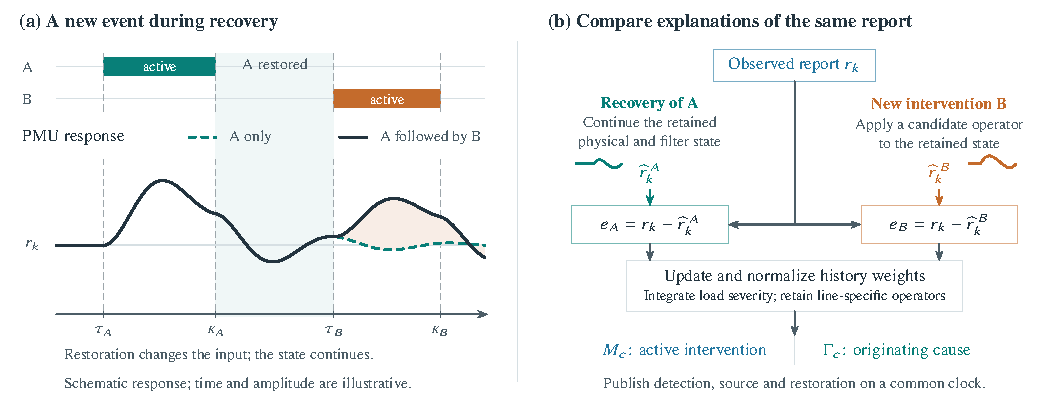
\includegraphics[width=.99\textwidth]{figures/generated/recovery_overview.pdf}
\caption{Attribution during recovery. (a) The event schedule and PMU response
share one clock. After B starts, the dashed curve continues A alone and the
solid curve includes B. (b) The same report enters separate innovation
calculations for recovery and a new intervention. History weights distinguish
active mass $M_c$ from originating-cause mass $\Gamma_c$. The traces and times
are schematic; the diagram shows two representative explanations within the bank.}
\label{fig:problem-method}\end{figure*}

The inference problem is to decide whether a new source is needed to
explain the incoming reports. Because the preceding response is still
evolving, the observation law depends on the earlier intervention.
Classical change
detection and isolation treats a single change of an otherwise stationary
law \cite{nikiforov1995generalized,lai2000sequential,tartakovsky2014sequential},
and the generalized-likelihood approach of Willsky and Jones detects jumps
in a fixed linear system \cite{willsky1976glr}. Power-system outage
detectors compare network hypotheses under quasi-static or linearized
models \cite{tate2008outage,chen2016quickest,rovatsos2017outage}, and
trajectory libraries diagnose faults from sparse PMUs
\cite{warner2023highfidelity}. These precedents motivate retaining a restored intervention as an explicit
competitor when attributing later observations in a switched DAE network.

We develop a bank of switched-DAE predictors that carries the estimated
state through restoration. Each history specifies a source, onset and
restoration time; load severity is integrated analytically. Separate active
and cause weights allow an intervention to end while its response remains
an explanation of later reports (Section~\ref{sec:narrative-method}).

We then examine two consequences of this construction. Nominal signature
energy describes source separation under the assumed plant and noise model,
and a reset analysis quantifies the innovation bias caused by discarding
physical state (Section~\ref{sec:theory}). A held-out comparison measures
timely attribution and extra alarms against a continuous physical GLR and
ExtraTrees at a common calibration budget
(Section~\ref{sec:recovery-comparison}). That comparison evaluates complete
procedures; isolating the benefit of keeping recovery histories requires a
further state-preserving control.

The evaluation covers a known catalog of sequential load and line
interventions. The supplement records auxiliary analyses and
reproducibility details.

\section{Related Work}
\label{sec:narrative-related}

\subsection{State Estimation and Physical Source Inference}
Unknown-input and DAE estimators recover electrical states despite
incomplete models or exogenous inputs
\cite{gillijns2007input,nugroho2022dae,katanic2024recursive}. Functional
observability asks whether a requested state quantity can be recovered
\cite{fernando2010functional,montanari2022functional}. Source inference asks
which intervention can explain the trajectory. Descriptor-model
diagnosability and nuisance-profiled tests formalize this distinction
\cite{eriksson2013diagnosability,scharf1994matched}.

Physical hypotheses support outage inference from phasor angles
\cite{tate2008outage}, Bayesian inference with uncertain states
\cite{zhao2014outages}, and sequential detection under stochastic operation
\cite{chen2016quickest,rovatsos2017outage}. Anguluri \emph{et al.} recover
sparse forcing locations, inputs and an unknown initial state using group
LASSO for linear dynamics \cite{anguluri2023group}. These are precedents
for source recovery; group LASSO is not an executed comparator in our
frozen campaign. Sensor placement also affects source distinguishability
\cite{jamei2020limits,conte2023fault,yildiz2025sparse}.

Recent learned reconstruction also targets sparse sensing. Pomarico
\emph{et al.}'s SHRED preprint evaluates dynamic-state reconstruction on
IEEE-39 from a limited number of PMUs \cite{pomarico2026shred}. Its target
is state reconstruction rather than the source/ON/OFF episode contract
here. Dey \emph{et al.} detect and localize distribution-network topology
changes from phasors using learned statistics, with hardware-in-the-loop
validation \cite{dey2026topology}. Neither sparse sensing nor change
localization alone distinguishes the present contribution. These are
adjacent tasks, not executed performance baselines in this study.

\subsection{Trajectory-Based and Sequential Diagnosis}
Warner \emph{et al.} compare simulated voltage/current fault trajectories
over a moving onset window and return candidate lines
\cite{warner2023highfidelity}. Their evaluated target is short-circuit
identification before clearing; load changes are an adverse-event test.
Our target follows load changes and line openings through restoration and
successive interventions. Physical trajectory libraries, remote PMUs and
retrospective onset scanning are shared ingredients. Their procedure was
not run on our data, so no numerical superiority is inferred.

The Adaptive Matrix CuSum derives sequential identification error/delay
results under specified observation laws \cite{warner2024matrix}.
Multiple-model filtering already propagates conditional state/mode
hypotheses \cite{blom1988imm}. The multiple-model multiple-hypothesis
filter maintains mode-sequence histories and adapts their number through
pruning and merging \cite{boers2005m3h}. Retaining histories or adapting
bank size is therefore not an original principle of our method.
Our pruned history bank uses these ideas,
but its approximate covariances, proposal screen and fitted startup context
do not inherit their general guarantees. The complete procedure evaluated
here makes retained recovery compete with later interventions and reports
timely attribution and alarm burden. These comparisons do not isolate
recovery memory from the other admission and publication rules.

\subsection{Learned Diagnosis and Physical Uncertainty}
Learned and knowledge-driven representations identify PMU disturbances and
assets \cite{pandey2020realtime,li2024knowledge,yildiz2024few}. We compare
two fixed ExtraTrees adapters from the SGSMA project. Their performance
tests transfer of those implementations, not the limits of all supervised
learning. A physical catalog and a fixed learned adapter have different
access to candidate-source responses. This comparison does not equalize
that information or establish a source-excluded generalization result.

Physical stochastic models support latent-state estimation
\cite{ensaf2023kernel,tartakovsky2023gp}, while joint DAE parameter inference
addresses uncertain generators and networks \cite{albustami2026dae}.
Our stream method uses a finite bank of constant network hypotheses.
Trajectory sensitivities and Gaussian evidence have also been combined
for Bayesian parameter inference in power-system DAEs
\cite{nagi2022trajectory}. Their use alone does not distinguish an event
attribution algorithm. The separate signature test examines a local event--context derivative;
it does not identify every plant parameter or replace the stream method
with an unrestricted joint estimator.

\begin{table*}[t]\centering\small
\caption{Closest inference contracts. Only Chen and the fixed ExtraTrees
adapters are executed comparators in the confirmatory stream campaign.
An untested capability is not an algorithmic impossibility.}
\label{tab:literature-capability}
\begin{tabularx}{\textwidth}{@{}lXXX@{}}\toprule
Route & Mechanism & Evaluated target & Role in this study\\\midrule
Chen / Rovatsos & Network likelihoods and sequential tests & Line outages; Rovatsos includes transients & Chen on persistent-line first decisions\\
Warner high-fidelity & Simulated V/I paths and onset search & Short-circuit line candidates & Closest trajectory precedent; no common-data run\\
Adaptive Matrix CuSum & Sequential diagnosis with error/delay analysis & One unknown distributional change & Statistical precedent; no inherited guarantee\\
IMM / M3H & Conditional filters, mode histories and mixture reduction & Hybrid switching-state estimation & Direct history-filter precedent; no common-data baseline here\\
DAE / stochastic-state estimation & Physical state and uncertainty models & States, unknown inputs or parameters & Components and adjacent tasks\\
Learned PMU diagnosis & Features or constrained representations & Event families and locations & Two frozen ExtraTrees references\\
Physical history bank here & Estimated-past-state paths and recovery & Successive catalog load/line events & Timely attribution, extras and restoration\\\bottomrule
\end{tabularx}\end{table*}

\section{Problem and Measurement Model}
\label{sec:narrative-problem}

At report $k$, inference uses measurements through $t_k=k/30$ to decide
whether a physical intervention occurred. Detection concerns its presence;
classification selects a physical operator; localization selects a bus or
branch. These outputs can become reliable at different times. We record
the estimated physical onset $\widehat\tau$ separately from the alarm and
diagnosis emission times.

Figure~\ref{fig:reference-event-types} introduces the broader measurement
phenomena using the reference record released with the SGSMA 2026
competition. Faults, line changes,
generation changes and load changes alter the physical network; missing or
corrupted reports alter observation integrity. The causal attribution test
addresses load changes and line openings with restoration; missing and
corrupted data are diagnosed by the integrity relations of
the supplementary integrity analysis. Faults and generation changes provide
context, not additional validated event classes.

\begin{figure*}[t]\centering
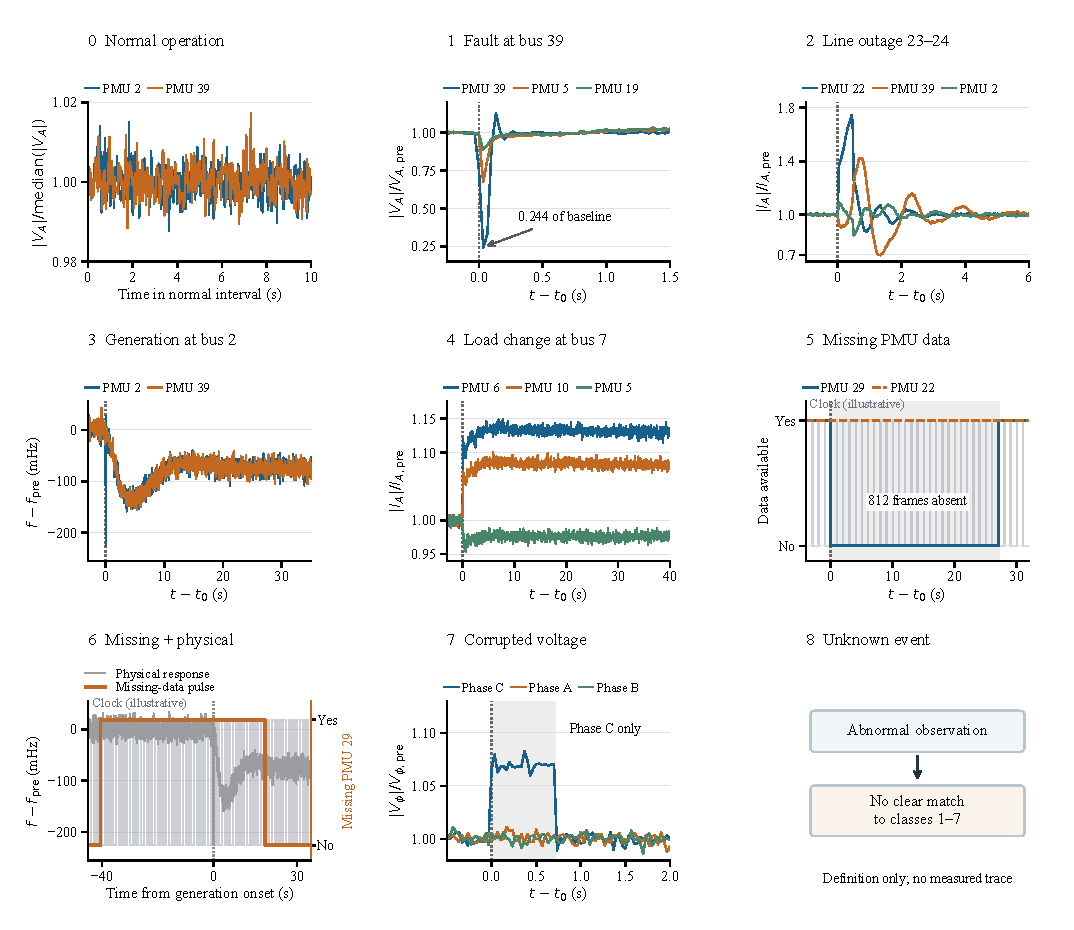
\includegraphics[width=.98\textwidth]{figures/generated/event_taxonomy_grid.pdf}
\caption{Representative signatures from the archived RAW0001 reference simulation of the SGSMA 2026 competition, arranged by label 0--8. Class 0 shows a normal interval; classes 1--5 and 7 retain the original trace values. Class 6 applies an illustrative data-loss mask from 0 to 30 s to the PMU 2 frequency trace (generation onset at 15 s): orange shows the available response and Yes level; blue marks No, while gray shows the response hidden during the gap, not a detector reconstruction. The mask is not the recorded outage interval. The gray clock trains in panels 5 and 6 are illustrative, not measured report timing. Class 8 is a definition schematic, not an observed trace or a validated bank output. Event traces are aligned to source labels for illustration only. Only load and line mechanisms enter the main causal evaluation.}
\label{fig:reference-event-types}\end{figure*}

The network has 39 buses, but the prescribed PMU set is
\begin{equation}
 \mathcal P=\{2,5,6,10,19,22,29,39\}.
 \label{eq:narrative-pmus}
\end{equation}
Voltage is measured at each PMU bus. Current is measured at a specified branch terminal, which can differ from that bus. The causal implementation uses 47 coordinates: eight voltage magnitudes, eight voltage angles, eight current magnitudes, seven current angles, eight absolute frequencies and eight ROCOFs, at 30 reports/s. BUS39 current angle is excluded because its interpretation remains partially validated. The BUS5 current terminal retains the provisional historical 5--6 assignment. These are declared measurement assumptions, not identities inferred from classification accuracy.

The exported magnitudes are in V and A, angles in degrees, frequency in Hz
and ROCOF in Hz/s. Internal centered coordinates do not replace the
definition of absolute frequency. These are reporting-rate phasor measurements;
waveform harmonics or THD are not measured by these channels.

The causal stream is exported from one balanced complex phasor per PMU:
phase A supplies the voltage and current magnitudes and angles. The CSV
exporter constructs B and C by equal magnitudes and angle offsets of
$-120^\circ$ and $+120^\circ$. Retaining A therefore loses no independent
phase information in these synthetic records; it is not measured
positive-sequence extraction or a model of unbalanced faults. The vector is
$y_k=(|V_A|_{\mathcal P},\angle V_A{}_{\mathcal P},
|I_A|_{\mathcal P},\angle I_A{}_{\mathcal P\setminus\{39\}},
f_{\mathcal P},\dot f_{\mathcal P})_k$.
The supplementary measurement table gives all eight current-terminal
assignments, polarities, gains and phase offsets. Products of voltage and
current measured at different terminals are power proxies.

% PROTECTED FIGURE: retain this single-column IEEE-39 diagram. See AGENTS.md.
\begin{figure}[t]\centering
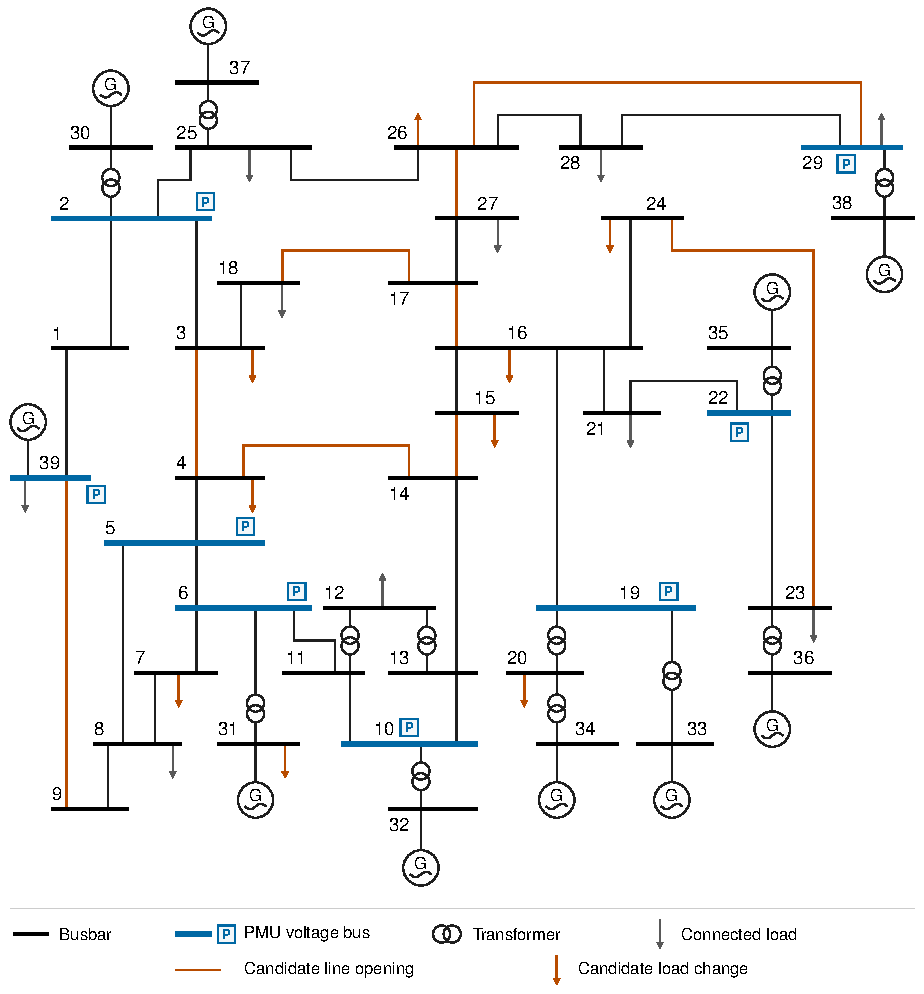
\includegraphics[width=\columnwidth]{figures/generated/narrative_topology.pdf}
\caption{IEEE 39-bus single-line diagram: 46 branches, 12 transformers and 10 generators. Blue bars and P marks locate the eight voltage PMUs. Orange branches and load arrows identify the nine line and nine load candidates; gray arrows denote other loads. Current terminals follow the separate measurement contract.}
\label{fig:narrative-topology}\end{figure}

The physical model is
\begin{align}
 \dot x&=f_q(x,z,u;\theta),&0&=g_q(x,z,u;\theta),\label{eq:narrative-dae}\\
 h_k&=H_q(x_k,z_k,u_k),\nonumber\\
 \eta_k&=F_M(\eta_{k-1},h_k;\theta_M),\nonumber\\
 y_k&=G_M(\eta_k,h_k;\theta_M)+b+\varepsilon_k.\label{eq:narrative-measurement}
\end{align}
Figure~\ref{fig:physical-measurement-chain} maps these physical and
measurement operations to the report consumed by inference.
\begin{figure*}[t]\centering
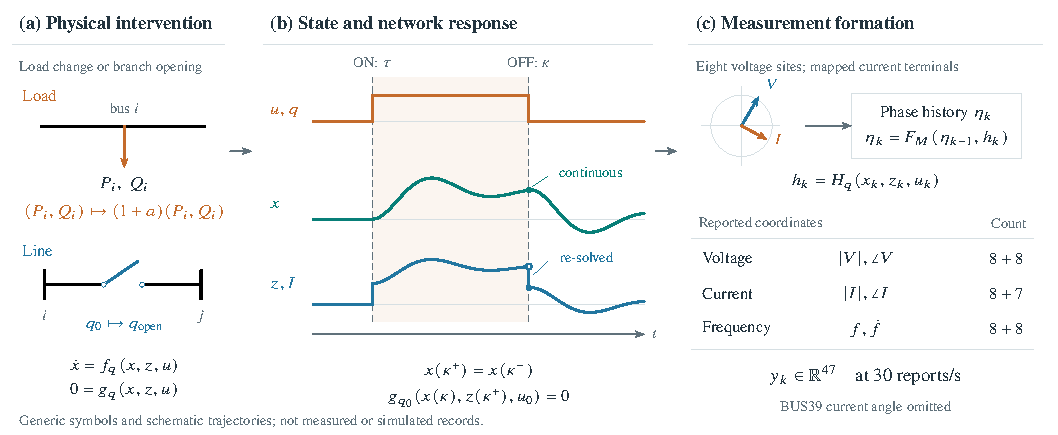
\includegraphics[width=.99\textwidth]{figures/generated/physics_measurement_chain.pdf}
\caption{Illustrative chain from load/line intervention to causal PMU report.
At OFF, the operator returns to baseline while $x$ and phase-history $\eta$
persist; algebraic voltages and currents are re-solved. Eight PMUs yield 47
coordinates at 30 reports/s; BUS39 current angle is omitted. Symbols and traces
are schematic. Phase B/C are reconstructed from A; raw waveforms and harmonics
are not inference inputs.}
\label{fig:physical-measurement-chain}\end{figure*}
Here $x$ contains machine and control dynamics, $z$ the algebraic network
variables, $q$ the topology/intervention mode, and $\theta_M$ the measurement
convention. $H_q$ selects electrical phasors; $\eta_k$ retains the causal
phase history used for frequency/ROCOF and the measurement-filter state.
The observation thus depends on an augmented state. Bus frequency comes
from phase evolution, not a machine's rotor speed. Instrumental noise is
generated by the noise model described in Section~\ref{sec:narrative-protocol}.

An intervention history is the discrete tuple
$h=(e,c,\tau,\kappa,\mathcal I)$: family, source, onset, restoration time
($\kappa=\infty$ for a sustained event) and, for a load, a severity interval
$\mathcal I$. The severity $a\in\mathcal I$ is a continuous latent variable
conditioned on $h$ and integrated in the evidence; a line opening has no
severity. A load changes its local P/Q setpoints by the common factor
$1+a$; a line opening switches its branch primitive. For the
supported impulse-free switches,
\begin{equation}
 x(\tau^+)=x(\tau^-),\qquad g_{q^+}(x(\tau^-),z(\tau^+),u;\theta)=0.
 \label{eq:narrative-switch}
\end{equation}
The algebraic voltage/current response may jump even though dynamic states remain continuous. Physical restoration reverses the intervention operator. It does not return the machines to their pre-event state, so electrical recovery can continue after OFF.

Switch-aligned reports use the consistent post-switch algebraic solution.
The local reduction requires an invertible algebraic Jacobian after fixing
the angle reference; the catalog excludes islanding line alternatives.
Successful solves and local residual checks validate the admitted cases,
not global regularity for arbitrary switching topologies.

\begin{table}[t]\centering\small
\caption{Scope of the executed causal component. The source is an intervention asset; it is not necessarily a measured PMU bus.}\label{tab:narrative-scope}
\begin{tabularx}{\columnwidth}{@{}lXX@{}}\toprule
Case & Physical operator & Executed claim\\\midrule
Normal & No intervention & Monitor after startup\\
Load & Local P/Q factor; optional restoration & Nine candidate buses\\
Line & Branch open; optional reclose & Nine candidate branches\\
Fault/generation & Different shunt/input/trip operators & Outside this causal test\\
Missing/bad data & Measurement-integrity mechanism & Parity diagnosis (supplement)\\
Unknown & Unresolved diagnosis & Not a new physical family\\\bottomrule
\end{tabularx}\end{table}

The generator stores event schedules and true states separately from the PMU stream. Inference receives the nominal network, permitted calibration and reports through the current time. It receives no source, switch time, true R/X realization or solver state. Initial operating context and noise scale are estimated from 300 startup reports; monitoring begins after a 12-s warmup. This startup estimate assumes an intervention-free prefix.

\section{Recovery-Aware Physical Attribution}
\label{sec:narrative-method}

At each report, the bank compares predictions from candidate intervention
histories (Fig.~\ref{fig:problem-method}(b)). Reduced state-space models carry
the physical and instrumental state forward; their dynamics and measurement
maps come from the network DAE. This avoids solving a full nonlinear
simulation for every candidate. Conditional filters account for uncertain
state and persistent model discrepancy, and the resulting evidence updates
the weights of the competing histories.

\subsection{Construct the Predictor From the Network}

Kirchhoff constraints and complex power connect sources to remote PMUs:
\begin{equation}
 I_{\rm bus}=Y_{\rm bus}V,\quad
 I_{{\rm term},r}=Y_{{\rm term},r}V,\quad S_i=V_i I_{{\rm bus},i}^{*}.
 \label{eq:narrative-electrical}
\end{equation}
Terminal rows retain orientation, line charging and transformer ratios.
A measured terminal current is not a nodal injection. A line opening
changes its branch primitive and terminal map; a load changes its admitted
P/Q input direction.

Each network hypothesis is linearized at the operating point
$(\bar x_\ell,\bar u_\ell)$ determined by its prefix-fitted load and
dispatch factors. For topology
$q$, the constructor holds $\bar x_\ell$ fixed and solves
$g_{\ell,q}(\bar x_\ell,\bar z_{\ell,q},\bar u_\ell)=0$.
On a regular index-one chart with a fixed angle reference, the derivatives
at that consistent point give, suppressing $\ell$,
\begin{align}
 \delta z&=-g_z^{-1}(g_x\delta x+g_u\delta u),\nonumber\\
 \delta\dot x&=c_q+A_q^{\rm red}\delta x+B_q^{\rm red}\delta u,\nonumber\\
 A_q^{\rm red}&=f_x-f_zg_z^{-1}g_x,\quad
 B_q^{\rm red}=f_u-f_zg_z^{-1}g_u.
 \label{eq:narrative-reduction}
\end{align}
Here $c_q=f_q(\bar x,\bar z_q,\bar u)$ can be nonzero after a line
opening even though the differential state is continuous.
For the instantaneous electrical observation map $H_q(x,z,u)$, the
corresponding output operators are
\begin{equation}
 C_q^{\rm red}=H_x-H_zg_z^{-1}g_x,\qquad
 D_q^{\rm red}=H_u-H_zg_z^{-1}g_u.
 \label{eq:electrical-output-reduction}
\end{equation}
The electrical offset is
$d_q^{\rm el}=H_q(\bar x,\bar z_q,\bar u)-H_0(\bar x,\bar z_0,\bar u)$.
Thus both the changed algebraic solution and the changed terminal map
enter the prediction. These operators propagate an unmeasured-source
perturbation to the selected
voltage and oriented-current channels. Branch stamps in $g_q$ and $H_q$ encode network connectivity;
eliminating unmeasured algebraic variables generally produces dense reduced
operators. A line switch changes both the voltage response and the terminal
operator in $H_q$. The implementation discretizes the admitted
switch modes and adds causal phase-history operators for frequency and
ROCOF. Inertia, controls and load law remain those of the fixed plant.

Exponential discretization integrates $c_q$ over each mode interval;
composition handles a switch within a report. After instrumental
augmentation, the resulting offsets enter $b_{\ell,q}$ and $d_{\ell,q}$ in
\begin{align}
 \xi_{k+1}&=A_{\ell,q}\xi_k+b_{\ell,q}+B_{\ell,q}a+w_k,\nonumber\\
 r_k&=C_{\ell,q}\xi_k+d_{\ell,q}+D_{\ell,q}a+v_k.
 \label{eq:implemented-predictor}
\end{align}
Here $r_k$ contains reference-corrected, scaled and instrument-whitened PMU coordinates, $\ell$ is a fixed
network hypothesis, and $\xi_k$ contains physical deviation states, phase
history and predicted measurement-filter memory. Observed colored-instrument
filters whiten measurements; their corresponding predictor memory is
deterministic. Additional latent AR states represent persistent discrepancy,
with preset quiet/load/line/recovery covariance and drift regimes. This
statistical discrepancy model is distinct from the plant equations.
$v_k$ denotes the remaining innovation. A load has scalar severity within
its specified P/Q direction. A line uses a switched operator rather than
a fictitious load-amplitude fit. States from different equilibria are not
interpreted as an absolute rotor-state mixture.
The supplementary section ``Implemented Predictor and Conditional
Uncertainty'' gives the affine construction and its code correspondence.

\subsection{Estimate Context From the Startup Prefix}

Each network hypothesis uses the same 300 startup reports to estimate
operating factors, reference phase and noise scale. Voltage/current
coordinates receive a constant discrepancy correction,
\begin{equation}
 \widehat b_\ell=\overline y_{0:299}-y_\ell^{\rm ref},
 \qquad b_{\ell,k}=\widehat b_\ell\quad(k\ge300).
 \label{eq:continuous-intercept}
\end{equation}
Angular differences respect wrapping and the common reference. Frequency
and ROCOF use empirical prefix centers. The correction remains fixed so it
cannot track a later load step and subtract its signature. This estimates
an observation discrepancy, not the true impedances. Prefix estimates
enter by substitution rather than through a full joint parameter posterior.

\subsection{Compare Unknown-Onset Histories}

The method retains ten seconds of past conditional states. Its
birth screen searches lags of 0--18 reports and proposes selected onsets;
it does not enumerate every onset in the 300-report history.
Each history specifies family, asset, onset,
restoration mode and severity. It starts from the stored conditional state
before its proposed onset. That state already contains any ongoing
recovery; an alarm does not reset the predictor to equilibrium.

For a retained load history, conditional Gaussian filtering yields a
residual $e$, severity response $s$ and covariance $S$. Unknown severity
has a truncated-Gaussian distribution inherited from previous reports:
\begin{equation}
 L_{h,k}=\int_l^u \mathcal N(e;sa,S)
             \operatorname{TN}_{[l,u]}(a;\mu,v)\,da.
 \label{eq:narrative-evidence}
\end{equation}
With $\Phi$ denoting the standard normal CDF, define
\begin{align}
 v'&=(v^{-1}+s^\top S^{-1}s)^{-1},\nonumber\\
 \mu'&=v'(\mu/v+s^\top S^{-1}e),\nonumber\\
 Z(\mu,v)&=\Phi((u-\mu)/\sqrt v)-\Phi((l-\mu)/\sqrt v).
\end{align}
The implemented local integral follows by completing the square:
\begin{align}
 \log L_{h,k}&=\log\mathcal N(e;0,S)+\tfrac12\log(v'/v)\nonumber\\
 &\quad+\tfrac12(\mu'^2/v'-\mu^2/v)
       +\log\frac{Z(\mu',v')}{Z(\mu,v)}.
 \label{eq:amplitude-evidence-main}
\end{align}
These standard identities are exact for the stated local conditional
model. Adaptive proposals, pruning and covariance approximations make the
complete bank approximate.

As in separate-bias filtering \cite{friedland1969bias}, the conditional
state mean is represented as $m_h+d_h a$; $d_h$ is the Willsky--Jones
signature of a unit severity propagated through the filter
\cite{willsky1976glr}. To make the filtering approximation explicit, let $T_o,J_o,g_o,u_o,j_o,v_o$ denote the
one-report transition and observation operators for switch $o$.
The code forms $e=r_k-J_o m_h-j_o$ and $s=J_o d_h+v_o$. With the shared
covariance $P_\rho$ for the current discrepancy regime $\rho$,
\begin{align}
 S_o&=R+J_oP_\rho J_o^\top,&
 K_o&=T_oP_\rho J_o^\top S_o^{-1},\nonumber\\
 m_h^+&=T_o m_h+g_o+K_o e,&
 d_h^+&=T_o d_h+u_o-K_o s.
 \label{eq:implemented-conditional-correction}
\end{align}
The amplitude distribution is updated by the same integral. Its truncated
variance $V_{a,h}$ differs from the Gaussian parameter $v_h$. The affine
conditional representation retains state--severity dependence:
\begin{align}
 \operatorname{Cov}(\xi,a\mid h)&=d_hV_{a,h},\nonumber\\
 \operatorname{Var}(\xi\mid h)&=P_\rho+d_hV_{a,h}d_h^\top.
 \label{eq:conditional-amplitude-covariance}
\end{align}
Conditioning on past reports is implicit. The shared $P_\rho$ solves the
nominal-operator Riccati equation of regime $\rho$; $S_o$ and $K_o$ are then
formed for each switched operator $o$. This is a steady-state
approximation, not an exact covariance recursion along each switched
history. At closure, the filter retains the augmented-state
mixture mean and records the amplitude/mean spread that it discards.
The supplement separates these approximations from the exact local
amplitude integral and states the covariance needed for a full mixture.

The rolling screen proposes histories; it is not another independent
observation. Replaying a suffix replaces its original no-new-event suffix
likelihood. The sequential update therefore counts each report once,
rather than repeatedly accumulating overlapping ten-second windows.

\begin{figure*}[t]\centering
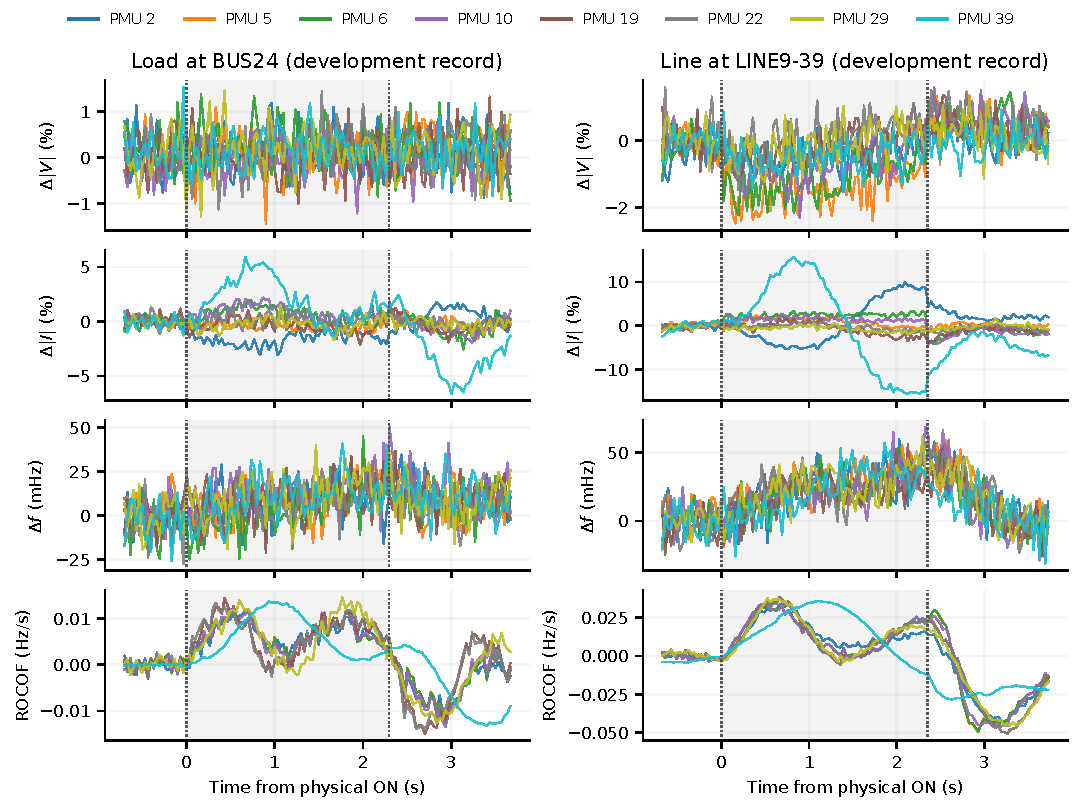
\includegraphics[width=.96\textwidth]{figures/generated/narrative_signals.pdf}
\caption{Simulated observations supplied to inference. One fixed development parent provides a load and a line example at all eight PMUs. Shading marks physical ON--OFF for evaluation only. Magnitude changes use the local pre-event center; frequency is centered for display while its exported channel remains absolute Hz. Source, severity and operating context affect the curves, so they are not universal class templates.}
\label{fig:narrative-signals}\end{figure*}

\subsection{Represent Fixed Network Uncertainty}

The bank contains nominal, global $\pm2\%$, and selected-branch $\pm3\%$
paired R/X hypotheses. Parameters stay constant within a hypothesis. Its
outer weight is updated with the one-step predictive density
\begin{equation}
 w_{\ell,k}=\frac{w_{\ell,k-1}p_\ell(y_k\mid\mathcal F_{k-1},\widehat b_\ell)}
 {\sum_jw_{j,k-1}p_j(y_k\mid\mathcal F_{k-1},\widehat b_j)},
 \label{eq:continuous-weights}
\end{equation}
\begin{equation}
 p_\ell(y_k\mid\mathcal F_{k-1})=\sum_{h'}\pi_{\ell,h',k-1}
 \sum_{h\in\mathcal T(h')}p_\ell(h\mid h')\,L_{\ell,h,k}.
 \label{eq:outer-predictive}
\end{equation}
The transition set $\mathcal T(h')$ contains continuation, restoration at
either half-report phase for an eligible active history, and a birth of
every catalog cell and severity interval at either phase from the
no-intervention history; the transition probabilities sum to one, which
the implementation asserts at every report. The density is evaluated
before any state is corrected and before retrospective proposals are
selected. Onsets proposed later for earlier reports change the inner
history posterior through suffix replay but do not re-weight
$w_\ell$; this is the one point where the outer and inner recursions
differ from a single joint posterior. Startup-fitting reports are not
scored again. The mixture covers a finite set of network alternatives
rather than a continuous impedance posterior.

\subsection{Keep Recovery as a Competing Physical Explanation}

Restoring an input or topology at $\kappa$ does not restore the pre-event
state: $x(\kappa^+)=x(\kappa^-)$. On a regular local post-restoration chart,
the difference from a same-context no-new-intervention trajectory obeys
\begin{align}
 \delta x_h(t)&\simeq\Phi_0(t,\kappa)\delta x_h(\kappa),\nonumber\\
 \delta y_h^{\rm net}(t)&\simeq C_0(t)\Phi_0(t,\kappa)\delta x_h(\kappa),
 \quad t>\kappa.
 \label{eq:recovery-response}
\end{align}
Here $y^{\rm net}$ denotes voltage/current coordinates before the instrument map.
Instrumental memory is retained as well. This local interpretation of known
dynamics explains why the reference after OFF is a predicted trajectory.

For conditional history mass $\pi_{\ell,h,k}$, define active and
originating-cause masses for an admissible family/source cell $c$:
\begin{align}
 M_{c,k}&=\sum_\ell w_{\ell,k}\sum_{h:c(h)=c}
       \pi_{\ell,h,k}\,\mathbf1\{h\text{ active at }k\},\nonumber\\
 \Gamma_{c,k}&=\sum_\ell w_{\ell,k}\sum_{h:c(h)=c}\pi_{\ell,h,k}.
 \label{eq:active-cause-masses}
\end{align}
A retained history can stop being active while its cause still explains
recovery. Later interventions compete with those histories. The
implementation stores 18 admissible cells, not every family at every bus.
After confirmed episode closure, explicit histories are compressed into
the retained state mean. Cause masses describe the current bank, not a
permanent ledger of all past interventions.

The implementation uses $M$ for active-event publication and $\Gamma$ for
source diagnosis. Their update weights are approximate because of pruning
and shared steady-state covariance approximations; they are not calibrated
posterior probabilities. A descriptive algebraic decomposition of
$\Delta M$ into within-model evolution and network-model reweighting is
given in the supplement; it does not enter the estimator's decision rule.

\subsection{Emit Separate Detection, Diagnosis and Restoration Messages}

An alarm is published when the active mass $\sum_cM_{c,k}$ exceeds 0.99 for
six consecutive reports. The rule has the structure of a Shiryaev
change-time threshold under the geometric prior
\cite{shiryaev1963optimum}, but pruning and covariance approximations make
0.99 an operational threshold on approximate mass, not a calibrated
posterior-probability guarantee. Six-report confirmation suppresses brief
excursions. OFF is published when the restoration mass exceeds 0.99 for 15 reports. The
diagnosis reports the family with the largest cause mass and its
highest-mass source; episode-replacement rules handle a different source
that begins before the previous episode closes. Every message records its
emission time and the last report used, so a diagnosis can be correct but
too late to precede physical OFF.

The nominal comparator is the same procedure with only the nominal network
hypothesis.

The per-report birth and restoration hazards are
$1-\exp[-(1/60)/30]$ and $1-\exp[-(1/30)/30]$, fixed during method
development before the independent schedules. They are deliberately
conservative: test interventions last 2--5\,s and are separated by 3--8\,s,
much shorter than the prior means of 60 and 30\,s. A low birth hazard raises
the evidence needed for an alarm by $-\log\pi_c$; Section~\ref{sec:theory}
shows that this margin is small compared with the available information.
Birth mass is split equally between load and line families, then uniformly
among sources within each family. Load severity has a zero-mean Gaussian
prior with standard deviation 0.15, truncated to $[-0.2,0.2]$ and integrated
over four intervals with boundaries $-0.2,-0.1,0,0.1,0.2$.
Each interval is a separate history with its own weight and truncated
amplitude distribution; its birth weight is the prior probability of that
interval. The physical operators are shared across these four histories.
For a fixed path with all four intervals retained, their weighted evidence
equals the single-interval integral.
This partition is a bank representation, not numerical quadrature or a
piecewise physical approximation.
After three reports, eligible active histories can produce OFF children
at either half-report position while inheriting state and severity.
After likelihood normalization, the beam retains the 96 highest-weight
recent histories, 64 older histories and at least one per occupied source;
their union is renormalized and discarded mass is recorded.
The supplement maps each operation to its implementation and lists the
complete publication configuration.

\subsection{Relation to Multiple-Hypothesis Filtering}
For a retained history $h$, let $p_\ell(h\mid h')$ contain the admitted
birth, continuation and restoration transitions. Before pruning, its
normalized evidence update has the standard form
\begin{equation}
 \pi_{\ell,h,k}\ \propto\ L_{\ell,h,k}
       \sum_{h'}p_\ell(h\mid h')\pi_{\ell,h',k-1}.
 \label{eq:history-bayes-update}
\end{equation}
This is the mode-sequence update of IMM and M3H filtering
\cite{blom1988imm,boers2005m3h}. Three features are specific to the present
problem: the modes are oriented electrical intervention operators derived
from the network DAE, histories carry a restoration time so that a restored
intervention remains a competing cause, and the output separates active
intervention from originating cause through \eqref{eq:active-cause-masses}.
Retrospective births reuse a stored pre-onset state, and confirmed closure
compresses histories into the retained augmented-state mean.

\subsection{Per-Report Algorithm and Computational Boundary}

\noindent\textbf{Algorithm 1: causal physical-history attribution.}
The inputs are the nominal model, the fixed method configuration and the
successive PMU reports; event truth never enters these steps.
\begin{enumerate}
\item Estimate operating context, common reference and noise scale from the
startup prefix. Initialize conditional states and retain the eligible past
states needed by retrospective proposals.
\item At report $k$, apply the fixed centering, scaling and instrumental
transformation. Propagate each retained physical/recovery history and its
conditional uncertainty to predict this report. Compute and save the outer
model predictive density before current-report screening and state correction.
\item Apply the short-lag birth screen using retained past states.
A proposed history starts before its selected onset; replay
replaces the corresponding likelihood suffix rather than adding it twice.
\item Score candidate histories and replayed suffixes before correcting
their states with the reports being scored. Integrate the allowed load severity and apply
the switched operator for a line hypothesis.
\item Correct the conditional states and severity distributions; update
network weights and the retained history bank using the fixed rules.
Preserve dynamic state and originating cause through restoration.
\item Aggregate active mass $M$ and cause mass $\Gamma$.
Apply the fixed alarm, diagnosis and OFF-publication rules. Store emission
time, estimated onset, family/source and the last report used.
\end{enumerate}
The nonlinear simulator constructs observations; this algorithm propagates
local switched predictors. Decisions use only reports already received.
Computation time is reported separately in Section~\ref{sec:narrative-results}.

\FloatBarrier
\section{Experimental Design}
\label{sec:narrative-protocol}

The primary experiment asks whether the causal bank can attribute successive load/line interventions without confusing recovery with a new event. Development, independent evaluation and an auxiliary source-resolution experiment answer different questions and retain separate denominators.

\begin{table}[t]\centering\small
\caption{Candidate assets fixed during method development, before the independent schedules. This is a known catalog rather than a representative sample of all network assets.}
\label{tab:source-catalog}
\begin{tabularx}{\columnwidth}{@{}lX@{}}\toprule
Family & Candidate physical sources\\\midrule
Load buses & 3, 4, 7, 15, 16, 20, 24, 26, 31\\
Lines & 3--4, 4--14, 9--39, 14--15, 16--17, 17--18, 23--24, 26--27, 26--29\\
\bottomrule\end{tabularx}\end{table}


\begin{table*}[t]\centering\small
\caption{Experimental populations and their purposes. Conditions and noise realizations repeat a physical parent rather than creating independent trajectories.}\label{tab:narrative-evidence}
\begin{tabularx}{\textwidth}{@{}lXXX@{}}\toprule
Population & Configuration & Main outcome & Interpretation\\\midrule
Continuous development & Three event parents, six interventions each; one normal parent; three network conditions & Timely family/source, extras and restoration & Open development evidence, not independent confirmation\\
Independent continuous evaluation & 18 event parents, six interventions each; 12 normal parents; three network conditions and two noise scales & Paired attribution, false alarms, delays and failures & Prespecified comparison of unchanged methods\\
Persistent-line evaluation & Nine lines, three parent repetitions; same network/noise strata & First stopping decision, source and censoring & Eligible comparison with published line-outage QCD\\
\IfFileExists{generated/ei_x02_macros.tex}{Supplementary signature test & \EIDictionaryCases{} dictionary and \EITestPhysical{} test trajectories; four loads; three common noise seeds & Nominal, reference correction and mixed-signature correction & Known ON/OFF and family; separate from causal accuracy\\}{}
Supplementary recovery geometry & 38 trajectories; four recovery histories and 12 correlated source-pair comparisons & Separation with known history and one uncertain severity direction & Supplied prior trajectory, onset, family and pair; separate from stream accuracy\\
\bottomrule
\end{tabularx}\end{table*}

The simulator is the IEEE-39 Julia/PowerDynamics research candidate. Each physical parent is integrated continuously, preserving differential states through ON/OFF. Its PMU reporting grid is separate from solver steps: a 120-s record contains 3601 reports per PMU and a 600-s normal record contains 18001, including endpoints. At a switch-aligned report the export uses the post-switch algebraic value. Measurement references, load law and stochastic instrument parameters are fixed across events. RAW0001 supplied retrospective calibration context, not independent test data.

The two development campaigns each contain three event parents with six successive load/line interventions and one normal parent, all 80 s long. Schedules are paired across nominal, in-bank R/X and mixed out-of-bank R/X conditions. Each campaign therefore has 18 unique interventions and 54 event realizations. Both campaigns are now development evidence. No interval or generalization claim treats those 54 realizations as independent events.

The five-model bank and its nominal version are frozen co-references.
Both ExtraTrees models were trained specifically for the causal load/line
catalog, using 32 earlier physical parents for training and eight for
development validation. Both training sets include normal operation and
all 18 candidate sources. The reference uses 846 causal features from
1-, 5- and 10-s windows; the short-window variant adds 611 features from
3-, 8- and 15-report windows. Each model has 400 trees with the same
predeclared hyperparameters. They inherit feature families from the SGSMA
project, but their fitted weights are distinct from the original hackathon
submission. These models and their adapters were frozen before the present
independent schedules; no retraining uses the current evaluation records.
All methods receive the same 30-fps observations. The supplementary
reproduction table records the training lineage and model hashes.

The learned adapter publishes a change after six consecutive identical
argmax labels. Its tree votes are uncalibrated scores. A missing timely
diagnosis can therefore reflect the representation, class competition or
temporal confirmation; conditional accuracy among emitted diagnoses does
not identify which mechanism caused an omission. The fixed-adapter
comparison measures transfer of these configured procedures rather than
an alarm-budget-matched architecture test.

The published physical comparator is Chen \emph{et al.}'s persistent single-line quickest-change detector \cite{chen2016quickest}. Its reduced-network covariance is marginalized to the observed PMU subset after inversion. Parallel CUSUM statistics stop at the first threshold crossing and select a line. Our declared research-plant adapter uses nonoverlapping angle increments at 15 Hz, a startup-only scale/drift estimate and the fixed nominal line catalog. Its white-injection/DC assumptions do not describe all simulated instrumental effects. We preserve both matched-law implementation checks and model-mismatch failures; no ARL guarantee is transferred to colored noise.

The eligible common test for Chen is one persistent line opening or a normal record. Its output has no load family or restoration operator. The independent campaign therefore separates continuous load/line episodes from persistent-line first-stop decisions. Early stops, wrong sources, omissions and horizon censoring remain visible.

For continuous events, an alarm is associated temporally before predicted family/source is inspected. The first unmatched alarm after ON is eligible up to the next ON, with the inherited 30-s cap. A timely joint decision requires the correct family and asset emitted before true OFF. Unmatched alarms are extras; false restorations and open episodes are reported separately. These definitions prevent an eventual correct answer from hiding a late diagnosis.

The independent campaign specifies 18 continuous parents, 27 persistent-line parents and 12 normal parents, with three R/X conditions and instrumental-noise scales of one and two. The 171 intended physical trajectories yield 342 observed records. Conditions represent nominal parameters, perturbations represented in the bank and mixed perturbations outside it. Solver and inference failures remain in the intended denominators. Comparisons use 10,000 paired parent-cluster resamples; repeated conditions/noise do not count as independent parents. Predictions are fixed before the evaluator opens reserved truth.

Logical decision delay is measured on report timestamps. Wall-clock cost is recorded separately with hardware, process concurrency and one-thread BLAS settings; parallel execution of independent records does not make a within-record inference method real-time. \IfFileExists{generated/c01_macros.tex}{The independent results are followed by a development example and the controlled component study.}{The independent evaluation is in progress. The following section reports completed development results only.}

\section{Results and Controlled Comparisons}\label{sec:narrative-results}
\subsection{Independent Evaluation: Timely Attribution and Alarm Cost}
\label{sec:c01-results}

The five-model bank makes \COneMixTimely{}/\COneMixTotal{} timely
family-and-source decisions with \COneMixExtras{} unmatched alarms on
event records, and its nominal counterpart \COneNomTimely{}/\COneNomTotal{}
with \COneNomExtras{}. These are paired replays of 108 interventions in 18
physical parents, not 648 independent events. On the 72 normal records
(42{,}336\,s, 11.8\,h of monitored time per method) neither bank raises an
alarm, which bounds the normal false-alarm rate below 0.26 per hour at 95\%
confidence (Poisson). Every matched diagnosis emitted before OFF names the
correct family and source; the timely misses are late or absent
diagnoses. Table~\ref{tab:c01-direct} and Fig.~\ref{fig:c01-main} give the
family split.

\begin{table}[t]\centering\small
\caption{Held-out continuous-stream decisions. Each family has 324 replays
of 54 distinct interventions; extras are unmatched alarms on event records.
The ExtraTrees adapters keep their original operating points.}
\label{tab:c01-direct}
\begin{tabular}{@{}lrrr@{}}\toprule
Method & Load & Line & Extras\\\midrule
Physical bank & \ReaderPhysicalLoad/324 & \ReaderPhysicalLine/324 & \COneMixExtras\\
Nominal bank & \ReaderNominalLoad/324 & \ReaderNominalLine/324 & \COneNomExtras\\
ExtraTrees & \ReaderETLoad/324 & \ReaderETLine/324 & \COneETExtras\\
ExtraTrees short & \ReaderETShortLoad/324 & \ReaderETShortLine/324 & \ReaderETShortExtras\\\bottomrule
\end{tabular}\end{table}

\begin{figure*}[t]\centering
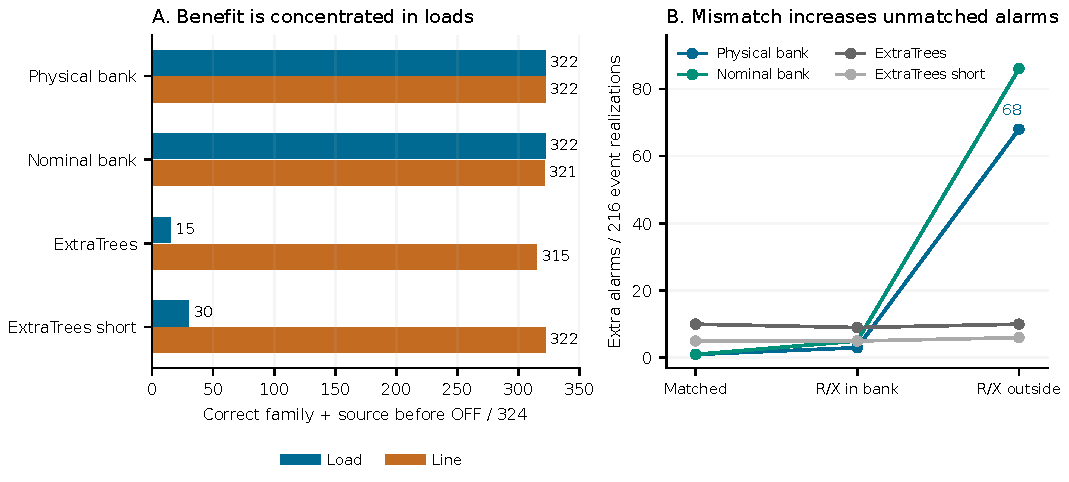
\includegraphics[width=.91\textwidth]{figures/generated/reader_c01_tradeoff.pdf}
\caption{Held-out continuous evaluation. (A) Timely correct family and source
by event family, with 324 paired replays per family. (B) Unmatched alarms on
event records for the two noise levels of each R/X condition (216 event
replays per condition). Each method keeps its own publication rule.}
\label{fig:c01-main}\end{figure*}

The extra alarms concentrate where the network model is wrong: 68 of the
72 occur when the true R/X perturbation lies outside the five-model bank,
68 alarms in 1.08\,h of out-of-bank monitored event-record time (about 63
per hour), against four in the other four strata together. Out-of-bank mismatch also produces the only
four timely misses. The supplement gives the paired parent-cluster
intervals; the physical bank's median alarm delay is about 0.27\,s in the
matched and in-bank conditions, comparable to the learned adapters
(0.19--0.30\,s).

We compare these delays retrospectively with Prediction~1. For the nominal bank on matched networks,
line alarms arrive after a median \RevObsLineDelay\,s, at the six-report
confirmation floor of \RevPredAlarmDelay\,s less the sub-report onset
phase, and doubling the noise leaves them unchanged. Load alarms arrive
after \RevObsLoadDelay\,s, again unchanged by doubled noise but about
\RevLoadExcessReports{} reports after the nominal signature reference crossing. Line delays are
consistent with the publication floor, while load delays exceed that
model-based reference.
The two ExtraTrees adapters recover lines (\ReaderETLine{} and
\ReaderETShortLine{} of 324) but few loads (\ReaderETLoad{} and
\ReaderETShortLoad{}). The diagnosis-time distributions in the supplement show that this is a
coverage failure: every load diagnosis the adapters do emit before OFF is
correct, but most load interventions receive none. A per-report audit on
four further matched records (12 load and 12 line interventions,
1{,}245 and 1{,}143 in-event reports) locates the failure before any
publication rule. During every load intervention the reference model's
per-report argmax is the normal class in all reports, and the median of
the largest true-class score is 0.09; during line interventions the true
line wins 96\% of the reports with median peak score 0.93. The short-window
variant ranks the true load first in only 2 of 12 load interventions. The
learned representation thus does not separate 3--14\% load changes from
normal operation, whereas the nominal physical signatures have large separation energies
for the same changes (Fig.~\ref{fig:theory-information}). The same pattern was already present in
their development validation (Section~\ref{sec:narrative-protocol}), so the
comparison shows that the physical bank recovers load interventions that
these particular adapters miss; it is not a test of the best attainable
learned detector at a common alarm budget.
In the persistent-line test, both banks and both adapters identify the
correct line first on all 162 openings. The adapter of Chen \emph{et al.}'s
quickest-change detector identifies 74/162; 66 records stop before the
opening and 22 afterward on a wrong line, and it stops on all 72 paired
normal records (first stop after 2{,}522\,s of cumulative normal exposure,
against 42{,}336\,s monitored without alarm by the other methods). Its
white-injection, quasi-static model does not describe the colored,
dynamically filtered measurements of this plant, so its threshold is far
from its nominal false-alarm rate. We therefore read this result as a test
of transfer under model mismatch, not as a ranking of quickest-change
detection. After the first identification, the two learned adapters raise
\PersistETExtras{} and \PersistShortExtras{} further unmatched alarms on the
same persistent records, against \PersistPhysicalExtras{} for the
physical bank. Stratified tables, failure ledgers, restoration outcomes and
censoring are in the supplement.

Table~\ref{tab:competition-metrics} restates the evaluation in the metrics
prescribed by the competition guide. Per-report detection F1 is 0.91 for
the bank and 0.58--0.64 for the learned adapters, whose precision is higher
because they alarm only on the line interventions. None of the methods
raises an alarm on the normal records. The bank has no trained weights:
its parameters are the network model, the noise model estimated from normal
data, and a few prior and publication constants fixed during
development. The nominal bank processes one
minute of PMU data in 48\,s on one CPU thread.
\begin{table*}[t]\centering\small
\caption{Independent evaluation in the metric vocabulary of the competition guide (648 interventions, 706\,min of normal records, three R/X conditions pooled). Detection is scored per report; Top-$k$ requires the correct family and source among the first $k$ candidates. Run time is per minute of PMU data on one CPU thread.}
\label{tab:competition-metrics}
\begin{tabular}{@{}lrrrrrrrr@{}}\toprule
Method & Precision & Recall & F1 & FA/min & Delay (s) & Top-1 & Top-3 & Run time (s/min)\\\midrule
Physical bank, five R/X models & 0.888 & 0.926 & 0.907 & 0 & 0.20 & 0.995 & 0.995 & 179\\
Physical bank, nominal model & 0.874 & 0.927 & 0.900 & 0 & 0.27 & 0.995 & 0.995 & 48\\
Submitted ExtraTrees & 0.938 & 0.424 & 0.584 & 0 & 0.27 & 0.509 & 0.509 & --\\
Retrained short-window ExtraTrees & 0.944 & 0.483 & 0.639 & 0 & 0.19 & 0.543 & 0.543 & --\\
\bottomrule\end{tabular}\end{table*}


\section{Development Comparisons and Worked Sequence}
\label{sec:narrative-results}

\subsection{Direct Transfer of the Submitted Hackathon System}
\label{sec:historical-transfer}

Before the confirmatory continuous study, the unchanged submitted ZIP
and an earlier physical estimator were executed on the same \HistoryWindows{}
windows: \HistoryEvents{} event realizations and \HistoryNormals{} normal windows.
Figure~\ref{fig:historical-transfer} preserves their actual family
confusions. The submitted ExtraTrees pipeline detected \HistoryETDetected{}
of the \HistoryEvents{} events, assigned the right family to
\HistoryETFamily{}, and the right family and exact source to
\HistoryETJoint{}. The earlier physical estimator obtained
\HistoryPhysicalJoint{}/\HistoryEvents{} for all
three quantities. Neither alarmed in the 28 normal windows. The source
result was checked against the submission's output CSVs, not inferred
from the family matrix.

\begin{figure*}[t]\centering
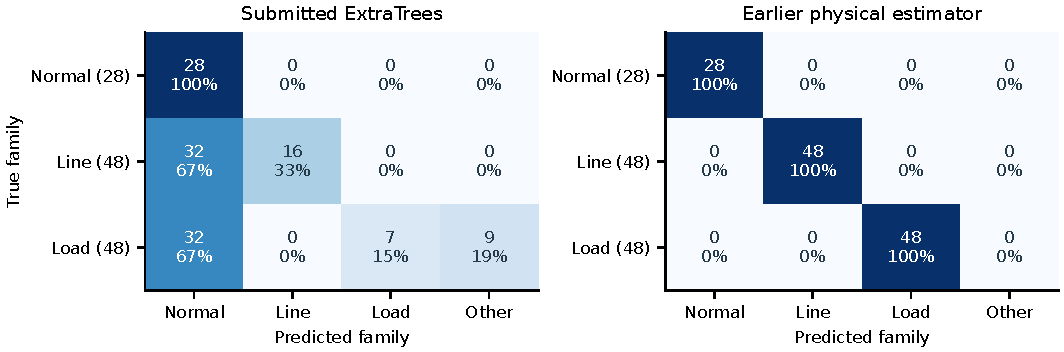
\includegraphics[width=.96\textwidth]{figures/generated/historical_transfer_confusion.pdf}
\caption{Historical development transfer on shared observation windows.
Cells show counts and row percentages. All out-of-scope predictions are
retained as ``Other''; the submitted system's nine such predictions were
the unknown-event label. This is a family matrix, not a localization
matrix. The physical comparator is an earlier estimator, not the final
continuous bank. The 96 event realizations reuse 36 physical event
trajectories; the normal windows come from six physical trajectories.}
\label{fig:historical-transfer}\end{figure*}

This comparison exposes a transfer failure of the delivered system on
the later simulator's load/line catalog. It does not show an official
hackathon-score improvement. The submitted model retains its broader
training domain and 30-s window rule, whereas the physical estimator
knows the simulator and its 12 candidate origins. These were development
cases, and the comparison permits both methods the same window endpoint.
The next study therefore uses separately trained causal ExtraTrees
comparators, successive events and a new frozen cohort. Its results must
be read as a second experiment, not as more independent repetitions of
the perfect development score.


\subsection{Following Successive Events Through Recovery}

The example in Fig.~\ref{fig:narrative-rolling} follows six physical
interventions without restarting the network. With matched R/X, all six
sources are identified before their OFF times. Under a network change
outside the bank, an extra bus-20 diagnosis precedes the real bus-31 load;
bus 31 is then diagnosed only after its physical restoration. The lower
panel shows the mechanism visible to the method: active bus-31 mass rises
late in the mismatched record. This is one development trajectory, not a
performance estimate.

\begin{figure}[t]\centering
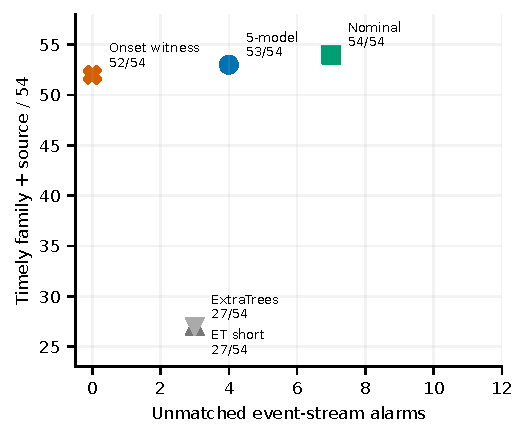
\includegraphics[width=\columnwidth]{figures/generated/narrative_tradeoff.pdf}
\caption{Development decision trade-off on 18 interventions replayed under three R/X settings. A stricter onset witness eliminates extra alarms but misses a true bus-16 load. The 54 plotted realizations share physical parents. These controls were not selected using the later sealed evaluation.}
\label{fig:narrative-tradeoff}\end{figure}

The development controls also show that deleting alarms is easy if true
events may be lost (Fig.~\ref{fig:narrative-tradeoff}). The stricter onset
witness has no extras but loses a real bus-16 intervention. The frozen
five-model procedure was therefore evaluated with its original publication
rule; no rule was revised from the sealed outcomes.

\begin{figure*}[t]\centering
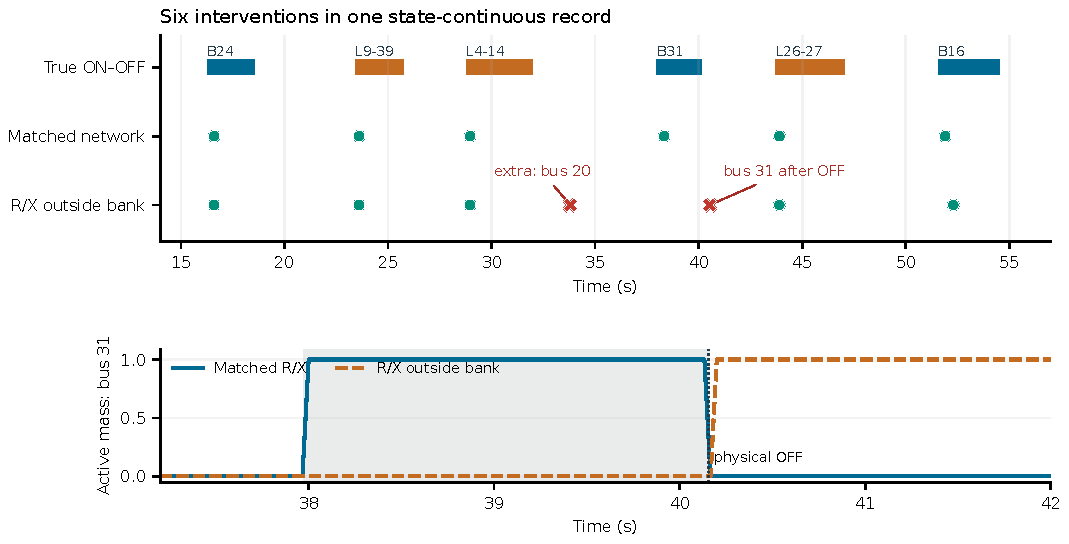
\includegraphics[width=.92\textwidth]{figures/generated/reader_episode_story.pdf}
\caption{One development sequence. Bars show reserved physical ON--OFF truth;
circles are correct diagnoses emitted before OFF; crosses mark an extra
bus-20 alarm and a bus-31 diagnosis emitted after OFF. Both lower decision
rows use the same physical bank under different R/X conditions. The lower
panel shows approximate active mass for bus 31: with R/X outside the bank,
the correct explanation becomes dominant only after restoration. Truth is
shown retrospectively and never enters inference.}
\label{fig:narrative-rolling}\end{figure*}

\subsection{Comparison With a Simpler Physical Procedure}
An earlier development control uses the same nominal physical and PMU
operators, one retained state and a short generalized likelihood-ratio
search. With a common six-report publication clock, it obtains
\SSSimpleTimely{}/\SSSimpleTotal{} timely decisions and
\SSSimpleExtras{} extras; the history mixture obtains
\SSMixTimely{}/\SSMixTotal{} with \SSMixExtras{}. This is an executed
physical comparator, separate from the later confirmatory cohort.
Different search, severity treatment and score semantics prevent it from
being a pure Bayes or memory ablation. Its equations and full table are
included in the supplement.

\subsection{Separating Severity Scoring From State Continuity}
\label{sec:component-study}

The continuous comparison evaluates complete procedures. To distinguish
two mechanisms within the physical bank, we fixed a subsequent $2\times2$
study: marginal amplitude evidence versus a bounded profile score, and
physical-state carry versus removal at inferred closure. The five network
models, observations, startup fits, operators, proposal rules and
publication thresholds are common to all four arms. Identical thresholds
do not imply identical false-alarm rates; both coverage and alarm counts
must be measured.

For one load history and amplitude interval $[l,u]$, write its accumulated
conditional log likelihood as
\begin{equation}
 \ell_k(a)=c_k+b_k a-\tfrac12 G_k a^2.
 \label{eq:ablation-quadratic}
\end{equation}
The original score uses $B_k=\log\int_l^u
\exp(\ell_k(a)-c_k)p(a)\,da$ with the existing truncated Gaussian prior.
The alternative uses
\begin{equation}
 \widehat a_k=\operatorname{clip}_{[l,u]}(b_k/G_k),\qquad
 Q_k=b_k\widehat a_k-\tfrac12G_k\widehat a_k^2,
 \label{eq:ablation-profile}
\end{equation}
with the constant-likelihood case treated separately. Each report adds
$B_k-B_{k-1}$ or $Q_k-Q_{k-1}$, so a rolling replay does not repeatedly
add the same suffix evidence. The conditional Gaussian amplitude/state
updates remain unchanged. Profile weights are normalized scores, not
posterior probabilities. This intervention tests the amplitude-scoring
choice, rather than removing every Bayesian calculation.
The existing Gaussian sufficient statistics supply
$G_k=v_k^{-1}-v_0^{-1}$ and $b_k=\mu_k/v_k$, removing the computational
prior precision before profiling. Fixed line-opening amplitudes and the
prior weights of amplitude intervals are unchanged.

At an internally inferred closure, the carry arm retains the projected
augmented state. The reset arm sets its 114 estimated physical-state
deviations to zero and retains instrumental/discrepancy coordinates,
covariance regime and network-model weights. This is an estimator
ablation: every observed record comes from the same continuous physical
trajectory. It does not test removal of all temporal information.

The protocol uses all 18 matched-network continuous parents at the
original noise level, plus the first three normal and persistent-line
parents by identifier. It was fixed before ablation outcomes, but the
underlying records had already been examined. Results are therefore a
posthoc mechanism study, with paired intervals over physical parents,
not a new independent confirmation.

\subsection{Effect of Preserving the Physical State}
\label{sec:controlled-ablation}
\begin{table*}[t]\centering\scriptsize
\caption{Controlled amplitude-score and physical-state-carry ablation. Same five-model bank and publication rules. All 18 continuous parents (108 events) are retained. Normal controls comprise three 600-s records with 588 s evaluated exposure each (1,764 s total; startup excluded). Delay is conditional on emitted matched diagnoses and must be read with the no-timely-diagnosis count.}
\label{tab:a01}
\begin{tabular}{lrrrrrr}\toprule
Procedure & Timely & Extras & Normal FA & False restorations & No timely & Delay (s)\\\midrule
Marginal + carry & 108/108 & 1 & 0/1,764 s & 1 & 0/108 & 0.267\\
Profile + carry & 108/108 & 1 & 0/1,764 s & 1 & 0/108 & 0.267\\
Marginal + reset & 75/108 & 166 & 0/1,764 s & 130 & 33/108 & 0.337\\
Profile + reset & 75/108 & 166 & 0/1,764 s & 130 & 33/108 & 0.337\\
\bottomrule\end{tabular}\end{table*}

\begin{figure*}[t]\centering
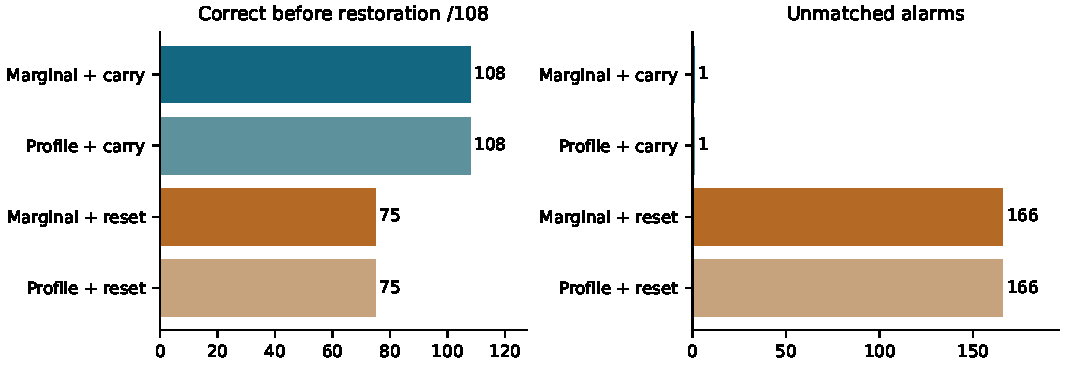
\includegraphics[width=.92\textwidth]{figures/generated/ablation_a01.pdf}
\caption{Severity-scoring and state-carry study on identical observations and five-model banks. The 108 interventions belong to 18 continuous trajectories. Thresholds are fixed, so the alarm rate may differ between arms.}\label{fig:a01}\end{figure*}
The nominal bank and the continuous GLR both carry physical state.
Their primary comparison therefore cannot identify the effect of resetting
it. In the fixed-threshold component study, resetting only the physical
coordinates reduced timely attribution from 108/108 to 75/108 and increased
unmatched alarms from 1 to 166 (Table~\ref{tab:a01} and Fig.~\ref{fig:a01}).
Marginal and profile severity scores gave the same outcomes within each
state treatment. The simulation itself evolves continuously in all arms.

\begin{figure}[t]\centering
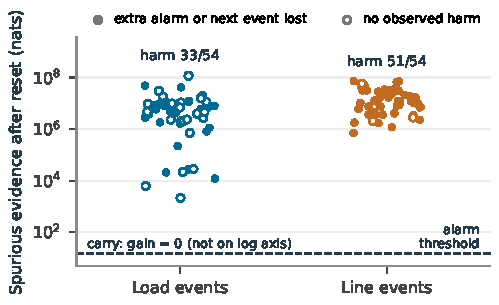
\includegraphics[width=\columnwidth]{figures/generated/theory_reset_cost.pdf}
\caption{Retrospective profiled energy gain after a state reset, \eqref{eq:reset-bias}, for the 108 interventions of the controlled study. Filled: an extra alarm in the following gap or a lost timely attribution of the next intervention; open: neither. The dashed line is the idealized score reference, not the publication threshold. Under matched noise-free continuation, carrying the state gives no positive gain over the null.}
\label{fig:theory-reset}\end{figure}

Fig.~\ref{fig:theory-reset} compares this outcome with the retrospective reset diagnostic. The
profiled energy gain exceeds $\lambda^\star$ after every intervention, by at
least two and up to seven orders of magnitude, and the reset arm is harmed
after \RevResetHarm{} of the \RevResetEvents{} interventions: an extra alarm
in the following gap or a lost timely attribution of the next one. Harm
occurs after \RevResetHarmLine{} line events and
\RevResetHarmLoad{} load events. The bus-31 events carry the smallest
profiled gain and are harmed after three of seven. The diagnostic shows
that reset leaves a residual that event candidates can explain. Its
magnitude alone does not determine the observed outcome: episode handling
and publication rules also matter. These are within-simulator contrasts at the
original thresholds; the two scores are compared at equal thresholds, not
at equal alarm rates.

\section{Discussion and Limits}
\label{sec:discussion}

\subsection{Physical-State Continuity as a Design Choice}
The strongest controlled result is the state-carry contrast. Physical OFF
restores an input or branch, while the machines retain their state.
Removing those estimated deviations at inferred closure substantially
worsens decisions on the same records. Marginal and bounded-profile
severity scores tie on the measured endpoints; both retain conditional
state estimation. This supports recovery-consistent prediction, without
showing that Bayesian marginalization is necessary for those endpoints.

The history bank gives a concrete way to represent the remaining response
and compare it with later interventions. Its complete operational behavior
is measured, but the reset control is deliberately severe. A continuous
physical observer without explicit recovery-history competition could
retain the same consistency. The open-development single-state GLR comparison gives preliminary
evidence against one such alternative, with different search and score
semantics. Independent validation under matched information and a common
calibration contract remains the key unresolved mechanism test.

\subsection{What Improved Relative to the Learned Reference}
The improvement concerns timely coverage of load sources under this
known-catalog simulator contract. Line coverage is comparable to the
short-window learned adapter. The physical method also issues more extra
alarms under network mismatch. The result is therefore a coverage--alarm
trade-off at fixed thresholds, rather than dominance at equal alarm rates
or a higher official hackathon score. Engineering physical features is
useful in the historical learned route; the physical bank additionally
computes how each candidate intervention should affect remote PMUs.
These routes have different access to source responses and training data.

A matched architecture comparison requires a physical continuous-state
control and a history bank with the same operators, together with a learned
baseline trained on the permitted catalog. Operating points must be chosen
on separate calibration records before a new test. The present comparison
preserves the frozen adapters and their failures. The two learned models
already saw all candidate classes during their earlier training; their
misses cannot be attributed solely to missing source labels or to an
unexamined scalar threshold.

\subsection{Model Correspondence and Measurement Scope}
The nonlinear generator and local predictors share the same research
plant family. Switched dynamics, nonlinear responses, noise and out-of-bank
R/X challenge the inverse model, but do not remove this shared-model
advantage. Independent dynamic-model or cross-simulator transfer remains
untested. All nine load and nine line candidates were inherited from
method development before the independent draw; they are a declared
catalog, not a representative sample of all 39 buses or all event families.

The eight-PMU terminal map is a research measurement hypothesis. BUS5
retains the provisional 5--6 assignment, and BUS39 current angle is excluded.
The synchronized channel grouping includes remote current terminals, so
it does not certify an installation of eight colocated voltage/current
PMUs. The observation model retains each terminal's actual location;
remote voltage--current products are power proxies.
The generator applies temporal and cross-PMU noise structure within each
signal family, but does not apply its archived cross-family factor
covariance. Frequency/ROCOF noise is added after phase estimation.
The experiment therefore does not validate a complete physical PMU noise
model, a producer's CT placement or exact reproduction of the historical
reference record. It also assumes an event-free startup and available PMUs.

\subsection{Approximation and Decision Uncertainty}
History pruning, shared regime covariances, plug-in startup estimates and
state-mean compression make the bank approximate. Its masses are
attribution weights under those approximations, not validated confidence
levels. The supplementary numerical checks verify the severity integral,
partition identity and conditional-state algebra under their local models.
Calibration of the nonlinear stream additionally requires pre-update
innovation diagnostics, interval coverage and sensitivity to pruning and
state compression. Existing instrumental whitening and latent AR states
address distinct components of dependence; their presence alone does not
establish predictive adequacy. Discarded mass is recorded by the
implementation, while a calibrated reliability and bank-size study remains
open.
Response fidelity and source discrimination also differ: sources may
remain close after fitting severity and context. The supplementary
context-signature and recovery-geometry controls preserve their null
source-decision results and do not supply an online identifiability
certificate. A useful extension would test whether a causal separation
margin predicts errors and delays before using it to justify abstention.

The measured research implementation runs below the input cadence.
Decision timestamps, computation delay and queueing must remain separate.
These results support further diagnostic development, rather than
protection or control deployment.

\section{Conclusion}
\label{sec:conclusion}

A restored load or line can leave a transient that resembles a new
intervention. The proposed bank predicts that transient from the carried
state and evaluates new source hypotheses against it. At a common
calibration target, the bank correctly attributed \RecBankTimely{}
interventions before restoration, compared with \RecGlrTimely{} for a
continuous GLR and \RecTreesTimely{} for ExtraTrees. During event records,
the three procedures emitted \RecBankExtras{}, \RecGlrExtras{} and
\RecTreesExtras{} unmatched alarms, respectively.

Resetting the physical state at inferred closure reduced coverage at fixed
thresholds. The difference between the complete procedures leaves open
how much explicit history retention adds beyond carrying state.
The evidence covers nonoverlapping load and line events from a fixed
catalog in one simulator family. Most unmatched alarms in the separate network-mismatch test occurred
under perturbations outside the five-model set. Independent per-PMU noise
reduced load attribution.


\FloatBarrier
\bibliographystyle{IEEEtran}
\bibliography{references}
% Public-source biographies authorized by the user on 31 October 2026.
% Evidence: docs/submission_successor_20261031/AUTHOR_PUBLIC_SOURCES.json.
% Keep author order. Verified institutional portrait sources are documented in
% figures/author_photos/PROVENANCE.md. Jorge and Yessica remain without photos
% until an attributable portrait is supplied.

% J2/J3: self-entered ORCID education and Uniandes thesis; no degree-conferral
% date, master's degree, or current university employment is asserted.
\begin{IEEEbiographynophoto}{Jorge Luis Mayorga Taborda}
studied electronic engineering at Universidad de los Andes, Bogot\'a, Colombia. His academic work has addressed distributed control using population dynamics, including applications to urban traffic systems.
\end{IEEEbiographynophoto}

% Y3/Y4: Uniandes thesis and IEEE-deposited publication metadata.
% No degree-conferral claim, current job title, or middle-name addition.
\begin{IEEEbiographynophoto}{Yessica Africano Rodriguez}
carried out undergraduate thesis work on photovoltaic integration at Universidad de los Andes, Bogot\'a, Colombia. Her published research includes co-simulation and stochastic assessment of photovoltaic hosting capacity in distribution systems.
\end{IEEEbiographynophoto}

% M1/M3/M4: Pitt institutional profile. Rank intentionally omitted because
% its contact card says Associate Professor while its narrative says assistant.
\begin{IEEEbiography}[{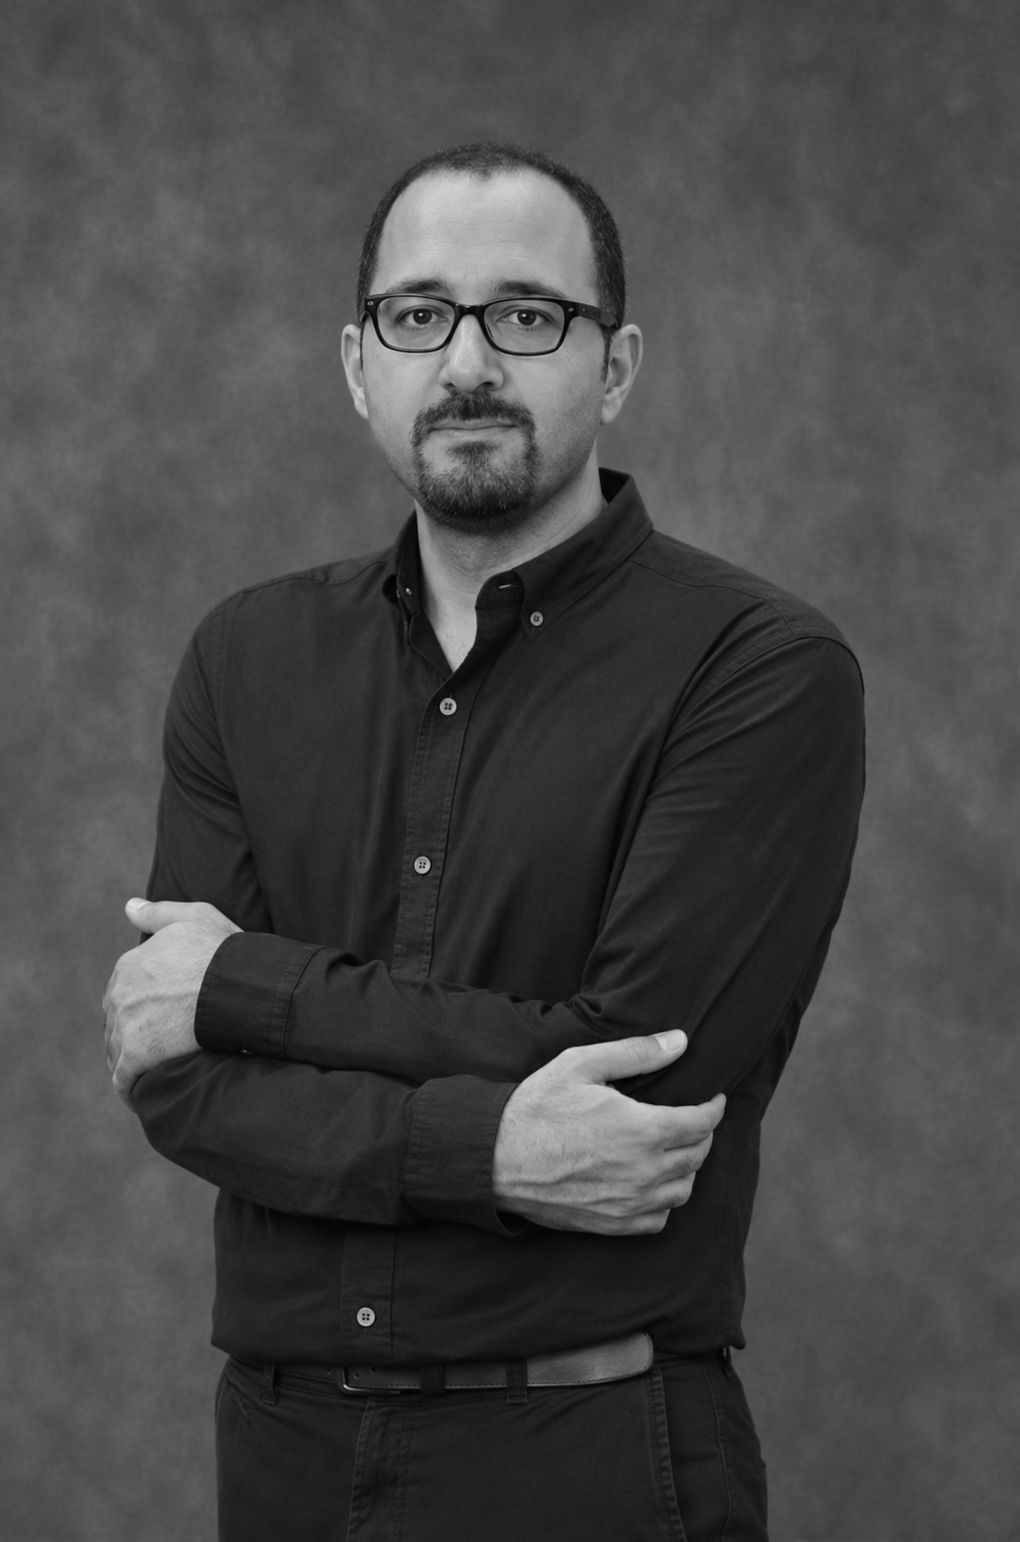
\includegraphics[width=1in,height=1.25in,clip,keepaspectratio]{figures/author_photos/masoud_barati_bw.png}}]{Masoud Barati}
received the Ph.D. degree in electrical engineering from the Illinois Institute of Technology in 2013. He is with the Department of Electrical and Computer Engineering, University of Pittsburgh, Pittsburgh, PA, USA. His research includes mathematical modeling and optimization of electric power systems.
\end{IEEEbiography}

% P1/P2/P3: current GWU faculty page.
\begin{IEEEbiography}[{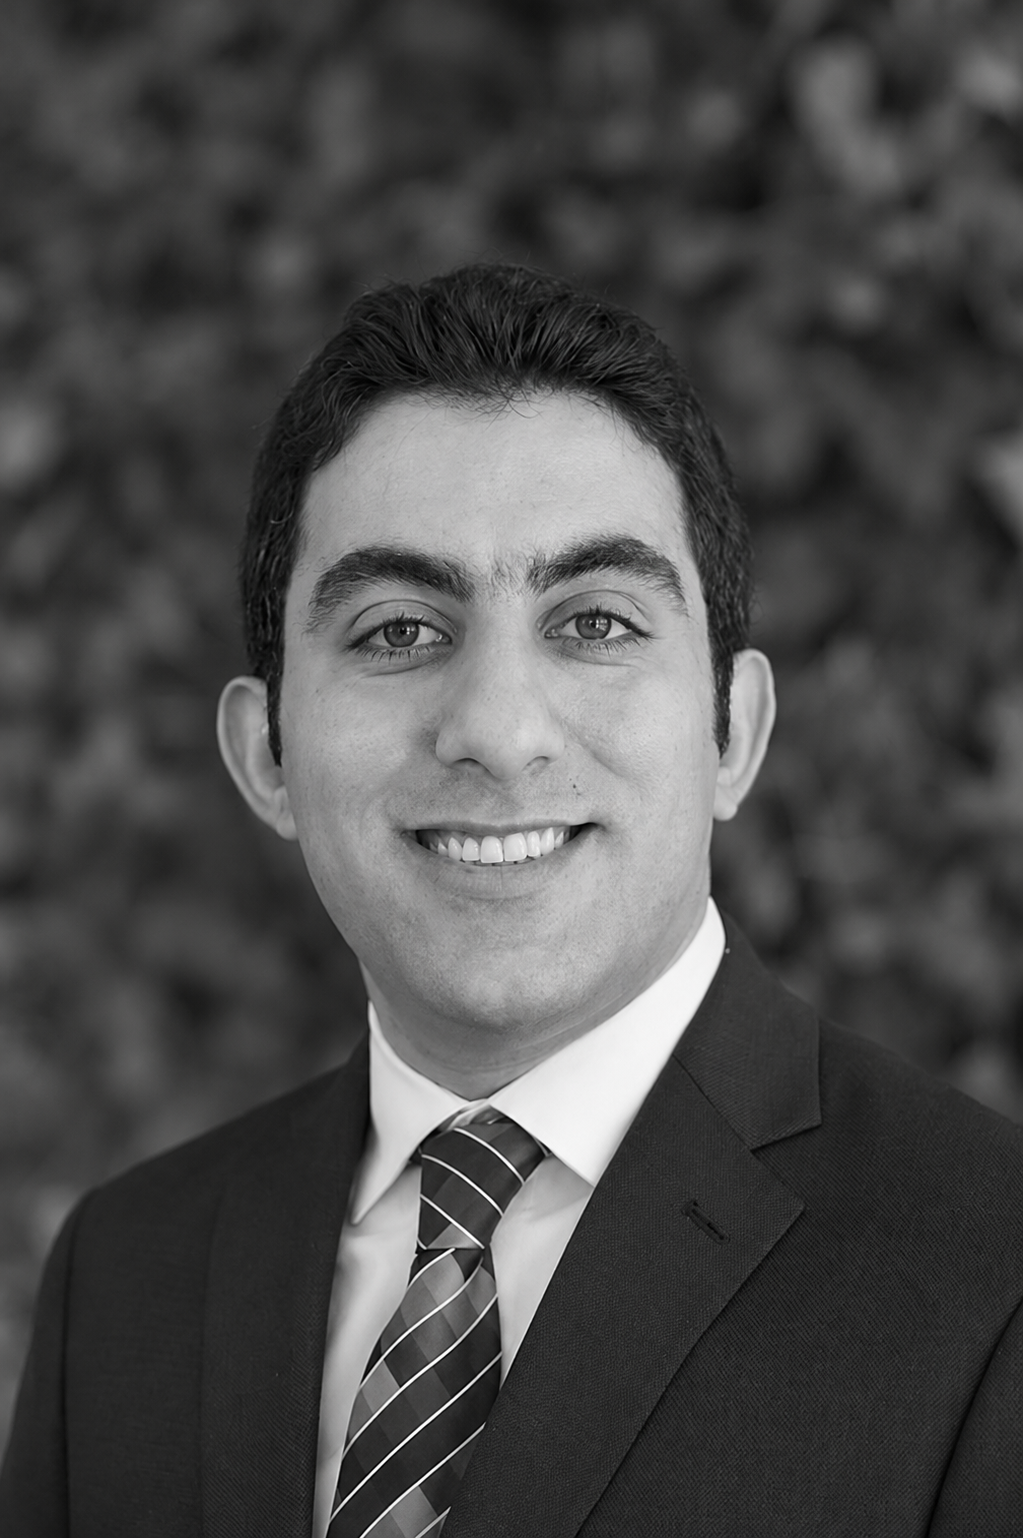
\includegraphics[width=1in,height=1.25in,clip,keepaspectratio]{figures/author_photos/payman_dehghanian_bw.png}}]{Payman Dehghanian}
received the Ph.D. degree from Texas A\&M University in 2017. He is an Associate Professor with the Department of Electrical and Computer Engineering, The George Washington University, Washington, DC, USA. His research includes power-system reliability, resilience, and data-informed decision-making.
\end{IEEEbiography}

% D1/D2/D3: La Sabana institutional profiles; broad institutional degree wording.
\begin{IEEEbiography}[{
\includegraphics[width=1in,height=1.25in,clip,keepaspectratio]{figures/author_photos/david_celeita_bw.png}}]{David Felipe Celeita Rodr\'iguez}
received the Ph.D. degree in engineering from Universidad de los Andes, Bogot\'a, Colombia. He is an Associate Professor and Director of Outreach and Engagement with the Faculty of Engineering, Universidad de La Sabana, Ch\'ia, Colombia. His research includes power-system protection, fault location, and real-time simulation.
\end{IEEEbiography}

\EOD

\end{document}
